\documentclass[12pt]{article}
\usepackage[margin = 1in]{geometry}
\usepackage[USenglish]{babel}
\usepackage{natbib}
\usepackage{multirow}
\usepackage{graphicx}
\usepackage{fancyhdr}
\usepackage{setspace}
\usepackage{verbatim}
\usepackage{booktabs}
\usepackage{amsmath}
\usepackage{lscape}
\usepackage{dcolumn}
\usepackage{subcaption}
\usepackage[title]{appendix}
\usepackage{xcolor}
\usepackage{todonotes}
\usepackage{titletoc}
\usepackage{longtable}
\usepackage[colorlinks=true,citecolor=red!50!black,urlcolor=blue!50!black,linkcolor=red!50!black]{hyperref}

\author{Patrick W. Kraft\footnote{Ph.D. Candidate, Stony Brook University, \href{mailto:patrick.kraft@stonybrook.edu}{patrick.kraft@stonybrook.edu}.
%I am indebted to Jennifer Jerit, Yanna Krupnikov, Jason Barabas, Stanley Feldman, Fridolin Linder, Hannah Nam, Scott Clifford, Peter DeScioli, Scott Bokemper, and participants of the Political Science Graduate Student Colloquium at Stony Brook University as well as participants at the panel of the 2015 Annual Meeting of the Midwest Political Science Association for helpful comments on earlier drafts of this paper. Furthermore, I thank Leonie Huddie for sharing the data for the telephone survey replication.
}}
%\date{}


\title{Morals Matter, But Not For Everyone
\footnote{An earlier version of this paper was presented at the 73rd Annual Conference of the Midwest Political Science Association, April 16-19, 2015. The manuscript and code are available on GitHub: \url{https://github.com/pwkraft/mft}.}
\\
\large{The Conditionality of Moral Foundations in Political Reasoning}}



\begin{document}
\maketitle
\doublespacing
\thispagestyle{empty}

\begin{abstract}
This study explores the role of morality in political reasoning by analyzing whether and how individuals evoke moral considerations when discussing their political beliefs. The proposed measurement approach identifies references to moral intuitions in open-ended responses using a dictionary previously validated in the literature on moral foundations. The analyses demonstrate systematic ideological differences in moral reasoning and extend previous findings by showing that the expression of moral considerations is conditional on individual political knowledge and exposure to political discourse. Moral arguments have a powerful influence on public opinion and political behavior but this relationship is most evident among the politically knowledgeable---implying that moral foundations are as much learned from the political world as they are innate.

\vspace{\baselineskip}
\noindent \textbf{Keywords:} Moral Foundations Theory, Political Reasoning, Ideology, Open-ended Survey Responses
\end{abstract}
\newpage
\setcounter{page}{1}

% ADD?
% Morality as a way for people to justify their political preferences
% I look at how people justify their political preferences and whether they make references to moral foundations
% More detailed discussion of why open-ended measures are useful to study social influence, political discussion, etc.?
% Why shoud we care about open-ended responses? Because that's how people describe their preferences! A survey is nothing but a highly structured conversation, so how people talk in a survey provides info for how they talk to each other (at least to some extent)

To what extent do the public's political beliefs have a meaningful structure? This question has been of frequent scholarly interest in political science and related disciplines, yielding an array of different perspectives. Early accounts emphasized how ordinary citizens lack consistent political attitudes and knowledge necessary to form meaningful ideologies \citep{converse1964nature}. However, with increasing levels of polarization and partisan sorting in contemporary politics \citep[e.g.][]{mason2014disrespectfully}, there has been renewed interest in systematic psychological and attitudinal differences between liberals and conservatives \citep{jost2006end}. One such area of research focuses on the differing moral concerns of liberals and conservatives. According to \textit{Moral Foundations Theory} (MFT), moral thinking is organized by five innate intuitions: harm/care, fairness/reciprocity, ingroup/loyalty, authority/respect, and purity/sanctity \citep{haidt2008moral,graham2011mapping}.\footnote{Subsequent accounts of MFT discussed alternative labels and the inclusion of further dimensions, such as Liberty/Oppression \citep[c.f.,][]{graham2013moral,haidt2012righteous}. However, the analyses presented here will only focus on the dimensions initially suggested in \citet{haidt2008moral}.} Liberals and conservatives differ in their relative emphasis on these foundations, with liberals prioritizing the foundations of harm/care and fairness/reciprocity, and conservatives endorsing all five dimensions more or less equally \citep{graham2009liberals}.

A series of studies builds on MFT and provides evidence for the influence of moral foundations on issue preferences \citep{koleva2012tracing, kertzer2014moral, low2015moral, clifford2015concerns}, candidate trait evaluations \citep{clifford2014linking}, and vote choice \citep{iyer2010beyond, franks2015using}. In contrast to this growing body of work documenting the political relevance of moral considerations, recent research casts some doubt on the theory's basic tenets by arguing that the foundations are less stable and more context-dependent than initially suggested (e.g., \citealt{smith2016intuitive}, see also \citealt{suhler2011can}). Yet, few studies have systematically investigated the conditionality of the relationship between moral foundations and political attitudes \citep[see][for a notable exception]{clifford2015concerns}. The present study attempts to fill this gap by directly examining the conditions under which individuals express moral concerns in political reasoning and judgment. 

The measurement approach proposed here uses a moral dictionary validated in previous studies \citep[e.g.,][]{graham2009liberals} to analyze individual verbatim responses to open-ended questions about political attitudes and preferences. Using open-ended rather than traditional closed items allows for a direct investigation of moral reasoning where the potential connection between morality and politics is not induced or facilitated by design. Furthermore, analyzing how individuals evoke moral considerations when they talk about politics is essential to understand the role of morality in political discussions and social influence. While the main analyses presented here are based on the 2012 American National Election Study, the method is validated using data from a telephone survey that varies the political context as well as the set of open-ended items included in the analyses.

The results reveal systematic differences between liberals and conservatives in the reliance on specific moral considerations when describing their political attitudes even without being cued to think about morality. These differences, in turn, affect political evaluations as well as voting behavior---even after controlling for a person's party identification. Most importantly, the overall reliance on moral foundations in political judgment as well as the respective ideological differences are conditional on knowledge and exposure to political discourse. Integrating a large-scale content analysis of individual media environments, the analyses proceed to show that individuals who are exposed to certain moral rhetoric are more likely to rely on corresponding moral considerations when discussing their own political beliefs. As such, even though the ideological patterns are broadly consistent with MFT, moral reasoning in the realm of politics is more context-specific than previous research suggests. From a methodological standpoint, the present study demonstrates how open-ended survey responses can be utilized to investigate the determinants of political reasoning. Specifically, I introduce methods to improve conventional dictionary-based approaches for the analysis of open-ended responses and showcase the integration of media content analyses to trace the influence of exposure to political discourse on individual response behavior.


\section*{Moral Foundations Theory}

Moral values serve as a source for coherence in political attitudes and they shape individual belief systems. As such, one major focus of the moral foundations framework is the relationship between moral values and political belief systems \citep[c.f.,][]{haidt2012righteous}. Liberal morals have been shown to focus on ``individualizing'' foundations, which include harm/care and fairness/reciprocity. Conservatives, on the other hand, also emphasize the remaining foundations of ingroup/loyalty, authority/respect, and purity/sanctity, labeled the ``binding'' foundations \citep{haidt2007morality,graham2009liberals}. Haidt and colleagues developed the Moral Foundations Questionnaire (MFQ) to measure individual differences in the emphasis of each foundation. The MFQ consists of a series of items that explicitly ask people to rate the relevance of different considerations when making decisions about right and wrong.\footnote{For example, one of the considerations is ``Whether or not some people were treated differently than others.'' High relevance of this statement is viewed as an indicator for the fairness/reciprocity dimension (c.f., \url{http://www.moralfoundations.org/}).} The questionnaire also asks individuals to indicate their level of agreement with statements that represent the values implied by the five foundations.\footnote{For example, respondents are asked to report their agreement with the statement ``I am proud of my country's history'' as an indicator for the ingroup/loyalty dimension.}

Relying on the MFQ, subsequent research extended the initial findings. For example, scholars showed that moral concerns predicted attitudes towards a wide variety of divisive political issues \citep[e.g.][]{koleva2012tracing,kertzer2014moral,low2015moral}. \citet{federico2013mapping} and linked moral foundations to individual social dominance orientation (SDO) and right-wing authoritarianism (RWA). Further research directly investigated the relationship between moral foundations and candidate preferences \citep{iyer2010beyond} or trait inferences about candidates \citep{clifford2014linking}. Moral foundations have also been shown to predict turnout \citep{johnson2014ideology} as well as voting behavior in the 2012 U.S. Presidential election \citep{franks2015using}. Overall, this research strongly supports the view that liberals and conservatives endorse different moral foundations and that these differences are related to political attitudes, evaluations, and behavior. Other studies, however, questioned some of the basic assumptions underlying MFT and argued that moral foundations cannot be viewed as stable traits \citep{smith2016intuitive,suhler2011can}. While it should be noted that these critiques are not without their own limitations\footnote{For example, the analyses presented by \citet{smith2016intuitive} relied on varying sub-scales of the MFQ, which might induce some of the temporal instability in moral foundations.}, they nevertheless raise the possibility that the relationship between ideology and moral reasoning is subject to more variability over time than previous research suggested. In order to reconcile the divide between the growing body of research highlighting the influence of moral foundations on political attitudes and work challenging those conclusions, it is necessary to directly investigate the conditions under which moral reasoning occurs when people think about politics.


\section*{The `Missing Link' to Political Reasoning}

Previous research has relied almost exclusively on the MFQ, which explicitly asks people to judge the relevance of particular moral considerations \citep[e.g.][]{graham2011mapping}. However, by directly asking people about the importance of considerations related to the five foundations, previous analyses presuppose an important link that requires more careful empirical investigation. More specifically, the MFQ does not allow for a direct examination of whether the connection between moral values and political ideology manifests itself when citizens reason about politics and evaluate political actors. Measuring moral foundations using the traditional measure therefore imposes constraints on the theoretical conceptualization of moral reasoning and the range of hypotheses that can be tested. Some scholars have criticized the MFQ because it does not ask people to make moral judgments per se \citep[e.g.][]{clifford2015moral}. Indeed, \citet[1031]{graham2009liberals} describe the reports on moral relevance as ``self-theories of moral judgment,'' rather than direct measures of judgment itself. Such abstract self-theories might, in turn, deviate from actual judgments in specific situations.

From a theoretical perspective, moral foundations are viewed as stable traits that affect attitudes and preferences regardless of potential individual differences and contextual effects. However, the incorporation of moral considerations in a specific political context could be much more variable. Previous research suggests that campaigns and elite communication can have important influences on individual moral reasoning. For example, \citet{clifford2013words} found that at the elite level, proponents and opponents of stem cell research place distinctive weights on moral foundations which in turn affected the public attitudes and the underlying considerations related to the issue. A subsequent study showed that elite rhetoric plays an important role in linking individual moral foundations with political attitudes, but only for those individuals who were most likely be exposed to it (\citealt{clifford2015concerns}; also see \citealt{day2014shifting}). While these studies do not contradict MFT, they cast some doubt on the notion that moral reasoning in politics is as a direct reflection of stable moral intuitions. 

The literature on moral convictions further suggests that moral reasoning in the realm of politics can be more variable than proposed by MFT. Skitka and colleagues argue that individuals hold moralized attitudes if they have a universal perception of ``right and wrong'' connected to the issue at hand \citep{skitka2005moral,mullen2006exploring,skitka2010psychology,ryan2014reconsidering,ryan2016no}. This view implies that there can be considerable variance in the degree to which moral considerations are raised between individuals and across issues. However, the MFQ measures moral foundations as general traits that are implicitly assumed to apply in any context. 

The present study addresses this gap by examining whether people utilize the foundations in their day-to-day political reasoning (i.e., without being prompted by the language of a questionnaire). Moving beyond the MFQ and measuring moral reasoning as the explicit expression of foundations allows us to directly examine the degree to which political attitudes are infused by morality. As such, this study investigates whether differences in moral reasoning between liberals and conservatives manifest themselves in a more unobtrusive context.

Insofar as moral intuitions play a role in political reasoning, citizens should rely on the moral foundations when reporting their attitudes towards political actors, even if they are not explicitly asked to do so. Thus, the first step of the analyses will be to replicate the findings connected to MFT and ideology using open-ended survey responses to general questions about political preferences. I expect that liberals will be more likely to spontaneously mention the moral foundations of harm/care and fairness/reciprocity than conservatives when evaluating political parties and candidates. Conversely, conservatives will be more likely to emphasize moral foundations of ingroup/loyalty, authority/respect, and purity/sanctity than liberals. Moral reasoning measured through open-ended responses is further expected to be politically consequential. The differences in the degree to which each foundation is emphasized should directly affect political preferences and vote choice consistent with the propositions of MFT.

After replicating the basic findings in the MFT literature in a more unobtrusive survey context that does not evoke issues of morality, the present study contributes to the literature by clarifying the conditionality of the foundations in day-to-day reasoning. Individuals who are exposed to the political process and resulting elite communications are expected to be more likely to incorporate moral considerations in their political reasoning because they adopt the respective arguments from elite discourse. Individuals who are not engaged in politics, on the other hand, might focus on other considerations when forming their preferences. The extent to which individuals rely on moral considerations when evaluating political actors is therefore not necessarily stable among individuals and across contexts. Rather, the tendency to emphasize moral foundations may be contingent upon individual levels of political knowledge, media exposure and political discussions. I expect that individuals who are more exposed to political discourse and more engaged in politics will be more likely to emphasize moral foundations when evaluating political parties and candidates than those who have less experience and are less politically engaged. Furthermore, these differences are expected to exacerbate the ideological divide in moral reasoning, especially if liberals and conservatives are exposed to divergent moral rhetoric.

The degree to which political attitudes are moralized as well as the ideological differences in moral reasoning cannot be investigated by relying solely on the MFQ. Instead, it is necessary to differentiate between a person's tendency to endorse a moral \textit{foundation} (as a stable trait, measured by MFQ), and moral \textit{reasoning} as the actual reliance on specific moral considerations and arguments in specific political judgments. Previous research has largely neglected this difference.


\section*{Measuring Moral Reasoning in Open-Ended Responses}

The present study is the first to explicitly focus on moral \textit{reasoning} by examining individual verbatim expressions of political attitudes and preferences. The analyses identify references to specific moral considerations when respondents discuss aspects that they like and dislike about political parties and candidates using the moral foundations dictionary created by \citet{graham2009liberals}. While the dictionary was initially used to analyze the content of liberal and conservative sermons, it was developed as a collection of general associations related to each foundation that could be applied in any context.\footnote{See Appendix~\ref{app:dict} for the full content of the dictionary.} For example, terms like ``protect'' and ``suffer'' indicate references to the harm/care foundation, ``equality'' and ``tolerant'' signal reasoning based on the fairness/reciprocity foundation, ``patriot'' and ``betrayal'' indicate reference to the ingroup/loyalty foundation, ``honor'' and ``respect'' signal considerations related to authority/respect, whereas ``integrity'' and ``disgusting'' indicate reference to the purity/sanctity foundation. Other studies in the domain of MFT relied on (variations of) the dictionary to investigate moral considerations in elite communication \citep[e.g. in news media coverage about stem cell research,][]{clifford2013words}, but to date no research has examined individual political reasoning in open-ended survey responses.

Based on the terms signaling each foundation in the dictionary, any text document can be scored according to its emphasis on the respective moral dimension. Conventional dictionary-based methods consist of the proportion of signal word occurrences in each document \citep[e.g.][]{graham2009liberals}:
\begin{equation}
\text{MFT}_{if} = \dfrac{1}{W_i} \sum_{t \in \mathcal{D}_f} w_{it},
\end{equation}
where $\text{MFT}_{if}$ denotes the score of document $i$ for foundation $f$, $W_i$ is the total number of words in document $i$, $t$ indicates a term in the set of signal terms in foundation dictionary $\mathcal{D}_f$, and $w_{it}$ denotes the number of occurrences of term $t$ in document $i$. In the analyses presented here, each document is an individual's verbatim response to a set of open-ended questions. As such, a respondent's MFT score for foundation $f$ is the overall proportion of words in the response that signal the respective foundation.

However, this conventional approach comes with an important drawback. While \citet{graham2009liberals} conceived the dictionary as applicable across contexts, some terms might be problematic when applied to verbatim survey responses. In particular, when respondents describe their attitudes towards political actors, certain words might be too ubiquitous to be regarded as an unambiguous indicator for specific moral considerations. For example, the moral foundations dictionary includes ``leader'' and ``honor'' as signal words for the authority/respect dimension. Should both words be considered equally indicative of the respective moral foundation? After all, if respondents describe their attitudes towards presidential candidates, they might be inclined to describe their qualities as \textit{leaders} irrespective of explicit moral considerations related to authority.

One way to address this problem using conventional methods would be to revise the dictionary and eliminate words that are deemed problematic. However, this leaves a lot of discretion to the researcher. Drawing on techniques developed in the field of information retrieval, the present study proposes an alternative approach. If it is the case that ``leader'' represents a term that is commonly used to describe presidential candidates (irrespective of moral considerations), then it should appear more frequently in open-ended responses across all individuals. Terms that are used by almost all respondents therefore provide less information about differences in their (moral) reasoning than terms that only occur in few responses.  Stated differently, if a specific moral word is mentioned by a large majority of respondents, it is more likely that the term can be used in multiple contexts and is therefore not necessarily unique to the moral domain.\footnote{For example, \citet{steyvers2003effect} relied on a similar reasoning in a recognition memory experiment that uses occurrence frequency of terms across documents as a proxy for their context variability.} In the analyses below, MFT scores are computed for a foundation by weighting each term in the dictionary according to its ubiquity across documents, which serves as a proxy for the term's discriminative information \citep[c.f. for example][]{manning2008introduction}:
\begin{equation}\label{eq:tfidf}
\text{MFT}_{if} = \dfrac{1}{W_i} \sum_{t \in \mathcal{D}_f} \left[ w_{it} * \log_{10}\left( \dfrac{N}{n_t+1}\right) \right],
\end{equation}
where $N$ denotes the total number of documents, and $n_t$ is the number of documents in which the term $t$ appears. The weight represents the inverse of the proportion of documents in which the target term appears.\footnote{This specification is usually referred to as tf-idf weighting and is commonly used in quantitative text analyses. The acronym tf-idf stands for ``term frequency - inverse document frequency,'' which refers to the rationale that the frequency of specific terms are weighted by the inverse of the frequency of occurrence across documents. See \citet[ch. 6]{manning2008introduction} for an introduction.} As such, terms that are ubiquitous across the entire corpus receive a lower weight, and terms that appear in only few documents receive a higher weight. The denominator in equation \eqref{eq:tfidf} includes $+1$ to ensure that it does not equal zero if a dictionary term does not appear in any of the documents.

The MFT score is a continuous measure that has a lower bound of 0 (document does not contain any dictionary terms) and is independent of document length (since it is based on relative occurrences). Higher scores imply larger proportions of dictionary terms in a document. Most importantly, however, words that appear in nearly all open-ended remarks affect MFT scores less than the words mentioned only by few respondents because ubiquitous words convey less information about differences across individuals. Overall, the MFT score provides a correction for potential distortions due to suboptimal terms in the dictionary while leaving its exact content outside of the researcher's discretion. Since nominal values of the MFT score above zero do not have a clear substantive interpretation, they are rescaled to unit variance.



\section*{Data, Variables, and Model Specification}

The analyses presented here are based on the 2012 American National Election Study, which contains two representative cross-sectional samples. One sample was conducted by computer assisted face-to-face interviews while the other sample is based on an internet panel group. Both samples are pooled in the analyses. While each consisted of a pre-election and a post-election wave, most items described below are drawn from the pre-election wave.\footnote{The open-ended items were included only in the pre-election wave. Accordingly, wherever possible, the set of explanatory variables was limited to the pre-election wave.}

The primary dependent variables (i.e., the MFT scores described above) are based on open-ended questions in which respondents were asked to report what they \textit{liked} and \textit{disliked} about either presidential candidate as well as the Republican and Democratic parties. More specifically, respondents were asked to list anything in particular that they like/dislike about the Democratic/Republican party as well as anything that might make them vote/not vote for either of the Presidential candidates and were probed by the interviewer asking ``anything else?'' until the respondent answered no. The responses to the eight open-ended like/dislike questions (evaluating both parties and both candidates) were aggregated for each individual and pre-processed by correcting spelling errors using an implementation of the Aspell spell checking algorithm in \texttt{R} (\url{www.aspell.net}).

Respondents were not included in the analysis if they failed to provide an answer to all open-ended items, or if the interview language was Spanish. Table~\ref{tab:app_mis} in the appendix provides an overview of the number of omitted cases. About 4\% of the interviews were held in Spanish and about 7\% of the respondents did not provide any open-ended response. Furthermore, Figure~\ref{fig:appB2num} in the appendix displays histograms of the length of the respondents' answers to all open-ended items. On average, the collection of all open-ended responses consists of about 75 words for each individual. Table~\ref{tab:sample} in the appendix additionally provides a sample of average-length responses that scored high on each of the moral foundations to illustrate how responses were processed.

Due to the fact that the MFT scores are bound at zero (i.e., none of the words in the dictionary appear in the response), individual response patterns are modeled via Tobit regressions for each of the moral foundations under consideration. The Tobit framework allows us to decompose the estimates into the effect on the probability of mentioning a specific foundation \textit{at all} as well as the degree of emphasis on the foundation given that it was mentioned by a respondent \citep[see][for details on the decomposition of Tobit model estimates]{mcdonald1980uses}.

The key independent variable used to predict the emphasis on each of the moral foundations, is \textit{political ideology}. Respondents were asked to place themselves on a seven-point scale ranging from extremely liberal to extremely conservative, which was transformed into dichotomous indicators for respondents who identified as liberals, conservatives, or moderates. Additional control variables included in the analyses are \textit{church attendance}, \textit{education} (college degree), \textit{age}, \textit{sex}, \textit{race} (African American), survey mode (online vs. offline), as well as the overall length of the individual responses in the open-ended questions (\textit{measured as logged number of words}). Furthermore, the 2012 ANES included the \textit{Wordsum} vocabulary test as a measure of literacy and verbal skill. It consists of a series of items asking respondents to choose a term that is closest to a target word. The Wordsum score consists of an additive index of correct responses in ten individual trials. The inclusion of the length of individual responses and the Wordsum score as control variables should account for potential confounding factors such as general effects of increased political literacy on the complexity of open-ended responses.

In order to examine the relevance and consequences of moral reasoning measured through open-ended responses, the MFT scores for each of the moral foundations are used as independent variables to predict political outcomes. The dependent variables considered here are \textit{candidate} and \textit{party evaluations} (measured as the respective feeling thermometer differentials), as well as \textit{voting behavior} (measured as a dichotomous indicator of vote choice for the Democratic rather than the Republican Presidential candidate reported in the post-election wave). In addition to the controls discussed previously, these analyses include measures of \textit{party identification}, which were recoded similarly to ideology.

The last set of analyses investigates whether the expression of moral considerations in political judgment is conditional on knowledge and exposure to political discourse. The factors that are expected to be related to references to moral foundations include \textit{political knowledge}, which was measured as the sum of correct answers to factual knowledge questions. The analyses also investigate the effect of \textit{political media exposure} and the frequency of \textit{political discussions} with friends and family members. Here, the analyses do not only examine the influence on individual foundations, but also consider whether these factors influence \textit{general} moral reasoning. This latter variable is measured as the sum of individual MFT scores across all dimensions (rescaled to unit variance after summation), which can be interpreted as a aggregate measure of how much respondents emphasize any moral consideration in their responses. Whenever appropriate, independent variables were rescaled to range from 0 to 1. Figure~\ref{fig:app_desc} in the appendix provides histograms of all independent variables included in different stages of the analyses.


\section*{Ideological Differences in Moral Reasoning}

Figure~\ref{fig:prop_ideol} presents a first descriptive overview of moral reasoning in open-ended responses. The figure displays the proportion of respondents who mentioned words that were included in the five different moral foundations dictionaries as well as their 95\% confidence intervals.\footnote{Note that the proportions are based on the subset of the sample that provided a response to at least one of the open-ended items, and for which the interview was held in English.} Since responses for each individual represent their likes and dislikes across all eight open-ended items, each proportion indicates the percentage of individuals who mentioned a signal word belonging to the respective moral foundation in any of his or her open-ended responses evaluating the parties or candidates.

\begin{figure}[ht]\centering
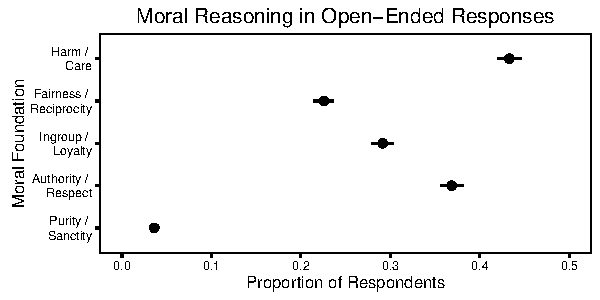
\includegraphics{../calc/fig/prop_mft.pdf}
\caption{Proportion of respondents mentioning each of the moral foundations in any of their open-ended responses, along with 95\% confidence intervals. The first two foundations are often labeled individualizing foundations, which have been shown to be more prevalent among liberals, while the remaining ones are described as binding foundations, which are more prevalent among conservatives.}\label{fig:prop_ideol}
\end{figure}
% ADD Note
% add note that first two are individualizing foundations, and the latter are binding foundations

The moral foundation most frequently mentioned is harm/care: About 42\% of the respondents mentioned at least one word included in respective dictionary. The second most frequently mentioned moral foundation is authority/respect with about 37\%. The proportion of respondents emphasizing ingroup/respect of fairness reciprocity is slightly lower with about 29\% and 23\%, respectively. Purity/sanctity, on the other hand, was almost never mentioned by any of the respondents. This finding is surprising, since other studies found the foundation to be an important predictor of divisive political attitudes \citep{koleva2012tracing}. This result suggests that the terms contained in the purity/sanctity dictionary might be too uncommon in the context of politics and therefore not relevant for attitude expression. Due to the very rare mentioning of the purity/sanctity dimension, the subsequent analyses will concentrate on the remaining four moral foundations.\footnote{Unfortunately, this issue cannot not be properly addressed by relying on weighting scheme employed here. The weights can correct for some distortions due to individual ubiquitous terms in the dictionaries, but it cannot compensate for the fact that the purity dictionary as a whole contains mostly words that are never mentioned by respondents.} Subsequent analyses focusing on the dimension of purity/sanctity in open-ended survey responses might necessitate a revision of the moral foundation dictionary.

Overall, Figure~\ref{fig:prop_ideol} shows that a substantial proportion of individuals evokes moral considerations when describing their political attitudes even when they are not explicitly asked about morality. However, we are ultimately interested in ideological differences in the emphasis of moral foundations in open-ended responses. As such, we now turn to a more in-depth analysis of the MFT scores as measures of moral reasoning.

We begin by estimating a set of Tobit regressions using ideology (and the control variables discussed above) to predict the individual MFT score for each of the moral foundations (excluding purity/sanctity).\footnote{The full estimates for this and all subsequent models discussed the remainder of the paper are presented in Appendix~\ref{app:tables}.} To reiterate, the MFT score measures the weighted proportion of moral foundation terms in an open-ended response. Figure~\ref{fig:tobit_ideol} compares liberals and conservatives while holding all other variables constant at their respective means. The effects of ideology (liberal - conservative) estimated in the Tobit model are decomposed into two parts: the left panel displays the change in probability of mentioning a specific foundation at all (i.e., probability of the MFT score to be larger than zero), whereas the right panel displays the expected change in the degree of emphasis on a foundation given that it was mentioned  (i.e., the change in the MFT score given that it is larger than zero, measured in standard deviations).

\begin{figure}[ht]\centering
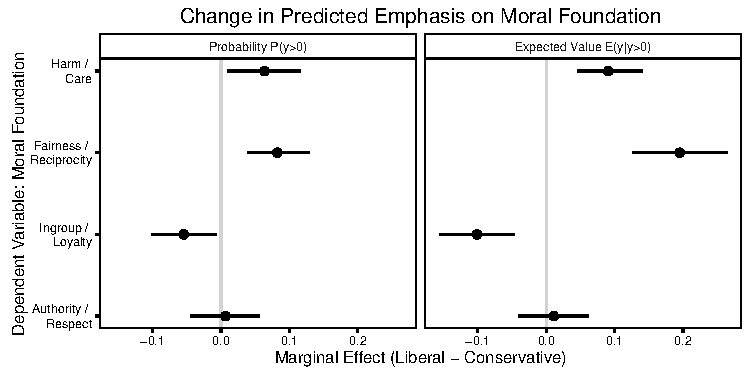
\includegraphics{../calc/fig/tobit_ideol.pdf}
\caption{Difference between liberals and conservatives in the probability of mentioning each moral foundation (left panel), and in the MFT score given that the foundation was mentioned (right panel), holding all other control variables at their respective means (along with 95\% confidence intervals). Positive values indicate that liberals are more likely to mention the respective foundation than conservatives (left panel), or emphasize it more than conservatives (right panel), and vice versa. Estimates are based on separate Tobit models for each foundation's MFT score. The dimension of purity/sanctity was omitted due to its low general prevalence in individual attitude expressions. Control variables include church attendance, education, age, sex, race, survey mode, response length, and the Wordsum vocabulary score. Full model results are displayed in the appendix, Table~\ref{tab:tobit_ideol}.
}\label{fig:tobit_ideol}
\end{figure}

Positive values denote a higher probability of mentioning the respective moral foundation (left panel) or a higher MFT score (right panel) of a response among individuals who identified as liberals, while negative values indicate a higher probability/higher score among conservatives. The effects are consistent with the the expectations of MFT for three out of four moral foundations. Liberals are significantly more likely to mention the foundations of harm/care and fairness/reciprocity. For respondents who identified as liberal as compared to conservative, the probability of referencing these two foundations is increased by about 6 percentage points. Furthermore, given that respondents mention these two foundations at all, liberals emphasize it more than conservatives when evaluating political parties and candidates. The MFT score for the harm/care foundation is about 0.07 standard deviations higher among liberals than conservatives. The effect is slightly larger for the fairness/reciprocity dimension. Conversely, being conservative increases the MFT score for the foundation of ingroup/loyalty by about 0.09 standard deviations. For the authority/respect dimension, we do not observe any significant differences between liberals and conservatives.

Taken together, the results are largely consistent with previous findings in the literature on MFT. Individuals evoke moral considerations when evaluating political parties and candidates without being explicitly asked about morality. Furthermore, there are systematic differences between liberals and conservatives in their reliance on binding and individualizing foundations \citep[see][for similar ideological differences when analyzing the content of life-narrative interviews]{mcadams2008family}. However, the fact that the authority/respect foundation showed insignificant patterns could suggest that the public's reliance on moral foundations may be more context-specific than previously thought.


\section*{The Political Relevance of Moral Reasoning}

A skeptical reader might argue that even if the ideological patterns are consistent with MFT, the expression of moral considerations might not be as strongly related to other forms of political behavior as latent moral foundations measured by the MFQ. In order to alleviate this concern, the analyses proceed to show that the expression of specific moral foundations in open-ended responses has important effects on political attitudes and behavior that match existing findings in the literature. Previous research relying on the MFQ has linked moral foundations to an array of political outcomes, such as candidate preferences \citep{iyer2010beyond} and voting behavior \citep{franks2015using}. Do we see the same patterns for explicit moral reasoning as compared to latent moral foundations?

\begin{figure}[ht]\centering
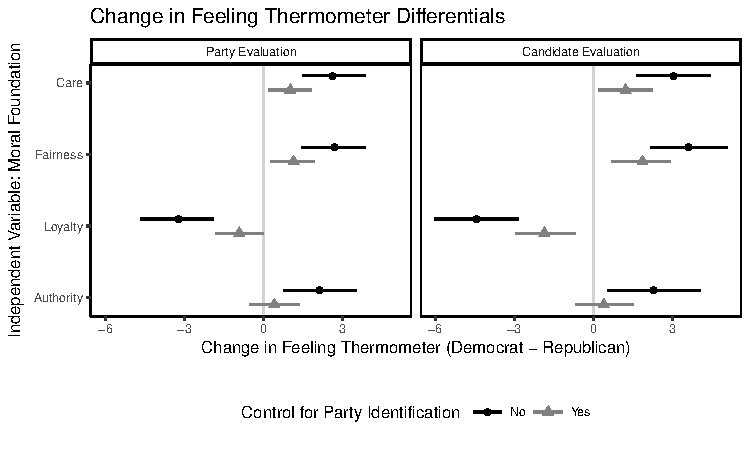
\includegraphics{../calc/fig/ols_feel.pdf}
\caption{Change in predicted feeling thermometer differential when MFT score is increased from its minimum (no overlap between dictionary and response) by one standard deviation, holding all other control variables constant at their respective means (along with 95\% confidence intervals). Positive values indicate that respondents who emphasized the respective foundation evaluated the Democratic candidate/party more favorably than the Republican candidate/party, and vice versa. Estimates are based on a single OLS model (using robust standard errors) including MFT scores for each foundation and gray triangles indicate estimates while additionally controlling for party identification. The dimension of purity/sanctity was omitted due to its low general prevalence in individual attitude expressions. Additional control variables include church attendance, education, age, sex, race, survey mode, response length, and the Wordsum vocabulary score. Full model results are displayed in the appendix, Table~\ref{tab:ols_feel}.
}\label{fig:ols_feel}
\end{figure}

As a first step, we examine the relationship of moral reasoning and attitudes towards political parties and candidates. Figure~\ref{fig:ols_feel} presents OLS estimates where feeling thermometer differentials between the Republican and the Democratic party (left panel) and between both Presidential candidates (right panel) are regressed on MFT scores for all moral foundations (including the control variables discussed above). Positive values indicate more favorable evaluations for the Democratic candidate or party and negative values indicate more favorable evaluations of the Republican candidate or party. The patterns are largely consistent with the previous results on ideological differences. Individuals who emphasize considerations related to harm/care, and fairness/reciprocity evaluate the Democratic party/candidate on average about 3 points higher than the Republican party/candidate (on a 100 point scale). On the other hand, if individuals emphasized the ingroup/loyalty dimension, they reported stronger preferences for the Republican party/candidate. Most of these effects are robust after controlling for individual party identification. Thus, in both analyses in Figure~\ref{fig:ols_feel}, we observe sizable and significant effects for the influence of moral reasoning. Interestingly, mentioning terms that belong to the authority/respect dimension appears to increase favorability towards the democratic party and candidate, which contradicts MFT. However, the effect disappears once party identification is controlled for.

\begin{figure}[ht]\centering
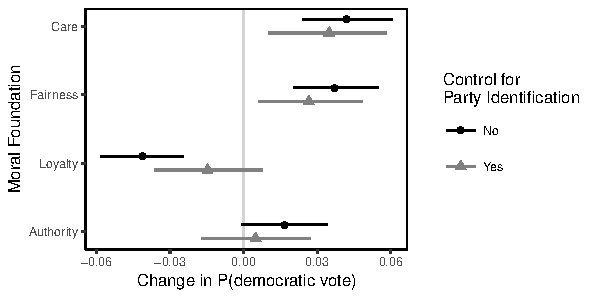
\includegraphics[scale=.9]{../calc/fig/logit_vote.pdf}
\caption{Change in predicted probabilities to vote for the Democratic rather than Republican candidate when MFT score is increased from its minimum (no overlap between dictionary and response) by one standard deviation, holding all other control variables constant at their respective means (along with 95\% confidence intervals). Positive values indicate that respondents who emphasize the respective foundation are more likely to vote for the Democratic candidate, and vice versa. Estimates are based on a single logit model including MFT scores or each foundation and dotted lines indicate estimates while additionally controlling for party identification. The dimension of purity/sanctity was omitted due to its low general prevalence in individual attitude expressions. Additional control variables include church attendance, education, age, sex, race, survey mode, response length, and the Wordsum vocabulary score. Full model results are displayed in the appendix, Table~\ref{tab:logit_vote}.
}\label{fig:logit_vote}
\end{figure}

Figure~\ref{fig:logit_vote} presents the changes in expected probabilities of voting for the Democratic (vs. the Republican) presidential candidate in the 2012 election for individuals emphasizing the moral foundations in their open-ended responses. The estimated probabilities are based on logit models including MFT scores for each moral foundation as independent variables (as well as  the remaining controls), which were held constant at their mean values when computing expected values. Again, the patterns are strikingly similar to the results presented thus far, and largely consistent with MFT. Individuals who emphasized moral considerations related to the harm/care and fairness/reciprocity foundations are more likely to vote for Barack Obama than for Mitt Romney. Respondents who emphasized the ingroup/loyalty foundation, on the other hand, were less likely to vote for Obama. 

The effects on political evaluations and vote choice might not seem large, but bear in mind that the measure of moral reasoning is based solely on the content of open-ended responses in which respondents were \textit{not} explicitly asked about morality. Yet, the moral considerations evoked by respondents were powerfully related to party and candidate evaluations as well as vote choice, even after controlling for strength of party identification and the length of individual responses. Overall, the analyses show that people's open-ended comments about both candidates and both parties are imbued with moral content and that these comments relate to political judgments in the manner predicted by MFT.


\section*{The Conditionality of Moral Reasoning}

Having shown that liberals and conservatives differ with regard to the moral foundations they emphasize when evaluating political actors and that these differences allow us to predict preferences and vote choice, we now investigate whether the reliance on moral considerations varies between individuals as a product of political knowledge and exposure to political discourse. Campaign exposure and discussions influence the degree to which political attitudes are moralized to the extent that individuals adopt moral rhetoric from elites and their peers. As such, we first focus on determinants of the general tendency to emphasize \textit{any} moral foundation by regressing the sum of MFT scores for each individual on political knowledge, political media exposure, and frequency of political discussions. Figure~\ref{fig:tobit_learn} depicts the respective effects when each independent variable is increased from its empirical minimum value to its empirical maximum value, holding all other variables constant at their means. Again, estimates are based on Tobit models that take into account the censoring of the moral reasoning measure and effects are decomposed into the probability of mentioning any moral foundation (left panel) as well as the emphasis on morality, given that any foundation was mentioned (right panel).

\begin{figure}[h]\centering
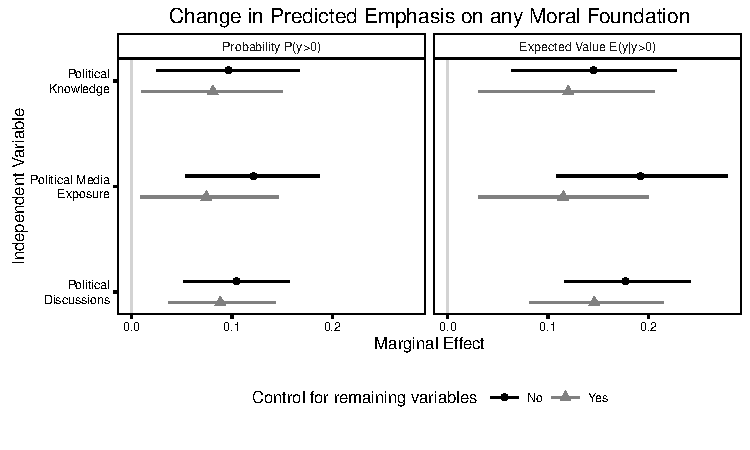
\includegraphics{../calc/fig/tobit_learn.pdf}
\caption{Change in predicted overall reliance on moral foundations depending on political knowledge, media exposure, and frequency of political discussions. The plot shows differences in predicted probabilities of mentioning any moral foundation (left panel) as well as in the summed MFT scores given that any foundation was mentioned (right panel), if each of the independent variables is increased from its minimum to its maximum value holding all other variables constant at their respective means (along with 95\% confidence intervals). Positive values indicate higher probability of mentioning, or stronger emphasis on moral foundations. Estimates are based on Tobit models and gray triangles indicate estimates while additionally controlling for the remaining variables presented in the figure. The dimension of purity/sanctity was omitted due to its low general prevalence in individual attitude expressions. All models include controls for church attendance, education, age, sex, race, survey mode, response length, and the Wordsum vocabulary score. Full model results are displayed in the appendix, Table~\ref{tab:tobit_learn}.
}\label{fig:tobit_learn}
\end{figure}

All variables considered here have a positive effect on the individual likelihood to mention as well as the respective emphasis on moral foundations when evaluating political parties and candidates. Higher political knowledge, higher exposure to political media and news, as well as more frequent political discussions increase the degree to which individuals rely on moral considerations. Thus, citizens \textit{learn} to embed moral reasoning in their political evaluations. While moral intuitions themselves might well be innate, the extent to which individuals make use of these intuitions when thinking about politics and evaluating political actors is context-dependent and subject to individual heterogeneity. It is worth reiterating that all models presented here control for education, logged overall response length, and the Wordsum score, which should account for potential confounding factors related to the respondents' eloquence when discussing their political attitudes.

The significant positive effect of frequent political discussions (even after controlling for political knowledge and media exposure), is especially interesting. Citizens who engage in frequent political arguments are more likely to use moral considerations when evaluating candidates and parties. This result suggests that morality serves as a rhetorical tool utilized to convince others of certain political views.\footnote{This conclusion is also supported by the finding that the reliance on moral considerations is more pronounced among individuals who engage in non-conventional forms of participation (e.g. signing petitions or wearing campaign buttons). Additional results are presented in the appendix, Figure~\ref{fig:tobit_part}.}

Beyond their effects on \textit{general} moral reasoning, we want to investigate whether the effects of political knowledge, media exposure, and discussions influence the systematic differences between liberals and conservatives in the emphasis on \textit{specific} dimensions. Consider again the results presented in Figure~\ref{fig:tobit_ideol}, which showed that liberals were more likely to emphasize the harm/care and fairness/reciprocity dimensions, while conservatives were more likely to emphasize the ingroup/loyalty foundation. In order to investigate whether the differences are conditional on political knowledge, media exposure, and discussions, the original models are extended by including interaction terms for each of the three variables that have been shown to influence the overall reliance on moral considerations. Based on these models, we can examine whether political knowledge, media exposure, and discussion frequency exacerbate the ideological divide in moral reasoning.


% ANALYSES REMOVED HERE

These results draw much more nuanced picture of the ideological differences in moral reasoning than previous studies. The patterns are only unequivocally consistent with MFT among politically knowledgeable respondents.\footnote{This is especially noteworthy given that many studies on MFT are based on opt-in samples collected through \url{www.yourmorals.org}, which potentially leads to biases towards higher education among respondents.} However, the picture is more complicated when looking at the influence of media exposure and political discussions. Exposure to political discourse increases the ideological divide on some dimensions but decreases it on others.

Explaining the patterns in Figure~\ref{fig:tobit_ideol_media}~and~\ref{fig:tobit_ideol_disc} requires a more in-depth analyses of the content of the media coverage as well as the nature of political discussions. It might be too simplistic to assume that exposure to news media and discussions always exacerbate the ideological divide in moral reasoning. In fact, such a pattern should only occur if liberals and conservatives are exposed to differential rhetoric that raises the respective moral considerations. For example, if a conservative regularly watches news programs that emphasize moral arguments related to individualizing foundations, he or she should not be \textit{less} likely to raise such considerations. In order to investigate this proposition, I make use of the fact that the 2012 ANES included a large array of items indicating whether individuals regularly watched various news outlets. For all media sources available, I downloaded the content of the coverage on either presidential candidates during the last month of the campaign (October 2012) from Lexis-Nexis and coded their emphasis on moral foundations using the same approach as for open-ended survey responses. The resulting MFT scores for each media source were median-centered and rescaled to unit variance.\footnote{In total, I retrieved the content of 28 media sources, such as the New York Times (print and online), CNN.com, or various Fox News Programs. See Figure~\ref{fig:media_desc} in the Appendix for a more detailed overview of the media outlets and their respective MFT scores for each dimension.} 

\begin{figure}[ht]\centering
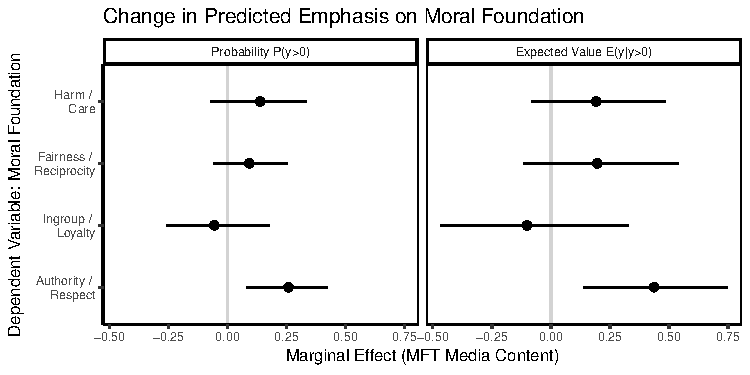
\includegraphics{../calc/fig/tobit_cont.pdf}
\caption{Effect of MFT content in individual media environments on the probability of mentioning each moral foundation (left panel), and on the MFT score given that the foundation was mentioned (right panel), holding all other control variables at their respective means (along with 95\% confidence intervals). For each moral dimension, the independent variable consists of the sum of MFT scores for media sources that are regularly watched/read by each respondent. Positive values indicate that individuals who consume media content that on average emphasizes the respective moral foundation more than other sources, are more likely to mention the respective foundation (left panel), or emphasize it more (right panel), and vice versa. Estimates are based on separate Tobit models for each foundation's MFT score. The dimension of purity/sanctity was omitted due to its low general prevalence in individual attitude expressions. Control variables include church attendance, education, age, sex, race, survey mode, response length, and the Wordsum vocabulary score. Full model results are displayed in the appendix, Table~\ref{tab:tobit_cont}.
}\label{fig:tobit_cont}
\end{figure}

Based on the coded content for each media source, I create a measure that represents the extent to which each individual's media environment emphasized any moral foundation. For each respondent in the ANES, I select the media sources he or she reported to watch/read regularly and computed the sum of the sources' MFT scores. Using this approach, I can analyze whether individuals who rely on media sources that emphasize a specific foundation more than other sources were also more likely to mention the respective moral dimension in their open-ended responses. Note that the analyses therefore only incorporate the moral content of each media source rather than its respective ideological leaning or the respondent's ideology.  The dependent variables are again MFT scores for the open-ended responses used previously and the models include the same controls. The results are presented in Figure~\ref{fig:tobit_cont}. Individuals who are mostly exposed to media sources that discuss moral considerations of harm/care put a stronger emphasis on related moral arguments in their open-ended responses describing their political attitudes. This finding is consistent with the results in Figure~\ref{fig:tobit_ideol_media}, which showed that media exposure exacerbates ideological differences on the harm/care foundation. Interestingly, we see a similar pattern for fairness/reciprocity: individuals who view political content that highlights the foundation are also more likely to mention related considerations in their open-ended responses. Media exposure therefore induces moral reasoning consistent with the source's content.

As such, media exposure should only foster the ideological divide in moral reasoning to the extent that the content of media sources exacerbates the respective patterns. This finding is quite encouraging given that \citet{haidt2012righteous} prominently argued that incompatibility in moral foundations are an important source for disagreements in politics. The results presented here suggest that differences in moral reasoning can be overcome if individuals are exposed to similar rhetoric in political discourse. For example, Figure~\ref{fig:tobit_cont} indicates that media content emphasizing fairness/reciprocity induces similar moral reasoning in attitude expression, but Figure~\ref{fig:tobit_ideol_media} shows that ideological differences on that foundation are only recovered among individuals with low media exposure. Taken together, the findings suggest that liberals and conservatives might select media sources that bridges the ideological divide on the moral foundation of fairness/reciprocity. While there is no data available to examine the same argument for the case of political discussion, the preliminary results presented above can be viewed as a strong case for subsequent investigations that incorporate the content of political discourse in the analysis of moral reasoning.

Overall, we can conclude from the analyses that whether researchers are able to recover systematic ideological differences in moral reasoning consistent with MFT is conditional on individual-level factors. Political knowledge, media exposure and discussion frequency not only affect general levels of moral reasoning but also moderate the ideological gap between liberals and conservatives. Some portion of the ideological differences in emphasis on moral foundations can therefore be described as a product of learning in the political environment. However, the nature of the relationship between political context and individual moral reasoning is complex and requires further investigation.


\section*{Examining Alternative Explanations}

The results discussed thus far revealed systematic ideological differences in moral reasoning when individuals discuss their political preferences. Furthermore, the expression of moral considerations in open-ended responses is politically consequential, but at the same time conditional on individual-level factors such as political knowledge. This interpretation, of course, relies on the crucial assumption that the dictionary-based approach for open-ended responses captures the theoretical concept of interest---\textit{moral} reasoning.

The remaining section briefly considers the possibility that this underlying assumption was not met and that the ideological divide observed throughout the analyses does not reflect differences in expressed moral foundations. Indeed, the terms in the dictionary may coincidentally recover unrelated differences in word choice between liberals and conservatives when discussing their attitudes towards parties and candidates in the 2012 U.S. Presidential election. For example, one prominent issue in the election was the Affordable Care Act, which might increase the likelihood of Democrats mentioning the term ``care'' and thereby increasing the emphasis on the harm/care foundation irrespective of underlying moral considerations. As such, the observed differences might be an artifact due to the nature of the questions under considerations as well as the specific political context of the presidential campaign.

In order to address these concerns, I replicated the main analysis using open-ended responses from a survey administered in a different political context. The survey was conducted via telephone with 594 adults aged 18 or older between early January, 2001 and July, 2003. The telephone numbers were a random-digit-dial (RDD) sample drawn from residents within a 25 mile radius of a large northeastern state university. As such, the survey was not conducted during a  major presidential election campaign. Furthermore, the survey uses a different set of open-ended items. Rather than asking about attitudes towards presidential candidates and both major parties, respondents were asked to describe liberals and conservatives as well as their respective beliefs in general. The coding and analyses are equivalent to those for Figure~\ref{fig:tobit_ideol}, although the survey did not contain the Wordsum scores (and varying survey mode) included as controls in the main analyses. The results are displayed in Figure~\ref{fig:tobit_ideol_lisurvey}.

\begin{figure}[ht]\centering
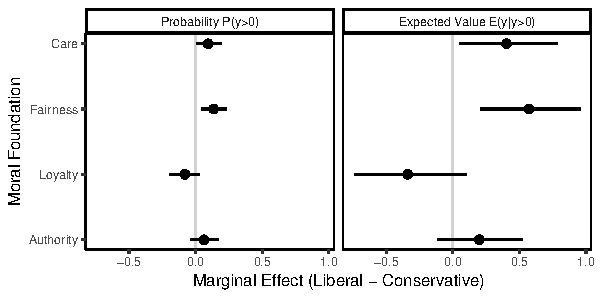
\includegraphics{../calc/fig/tobit_ideol_lisurvey.pdf}
\caption{Replication of main model (c.f., Figure~\ref{fig:tobit_ideol}) using RDD sample from residents within a 25 mile radius of a large northeastern  state university. Figure displays difference between liberals and conservatives in the probability of mentioning each moral foundation (left panel), and in the MFT score given that the foundation was mentioned (right panel), holding all other control variables at their respective means (along with 95\% confidence intervals). Positive values indicate that liberals are more likely to mention the respective foundation than conservatives (left panel), or emphasize it more than conservatives (right panel), and vice versa. Estimates are based on separate Tobit models for each foundation's MFT score. The dimension of purity/sanctity was omitted due to its low general prevalence in individual attitude expressions. Control variables include church attendance, education, age, sex, race, and response length. Full model results are displayed in the appendix, Table~\ref{tab:tobit_ideol_lisurvey}
}\label{fig:tobit_ideol_lisurvey}
\end{figure}

The patterns are strikingly consistent with previous results. Liberals are more likely to emphasize the foundations of harm/care and fairness/reciprocity. The result for the ingroup/loyalty dimension, however, do not reach conventional levels of statistical significance. Additional analyses reveal that the ideological differences in moral reasoning are mostly due to the fact that individuals who identify as liberals emphasize the foundations of harm/care and fairness/reciprocity more strongly than conservatives when describing their ingroup (i.e., other liberals and their beliefs), while conservatives emphasize the foundation of ingroup/loyalty more strongly than liberals when describing their ingroup (results available upon request). The fact that the same basic ideological pattern can be recovered in a survey that was conducted in a different political context (non-election period, Republican administration), employed a different survey mode (phone interview), and relied on a different set of open-ended survey questions (asking about liberals and conservatives and their respective beliefs), provides further support for the argument that the MFT dictionary allows us to recover basic moral considerations in political reasoning.


\section*{Conclusion}

There is much more to be learned about the relationship between moral foundations and broader political attitudes and ideology \citep[e.g.,][]{feldman2013political}. To fully understand how political views are rooted in morality, researchers need to take a closer look at the conditions under which citizens express moral considerations in the context of politics. In contrast to previous accounts of MFT, I argue that the reliance on moral reasoning is moderated by political knowledge, media exposure, and political discussions. Not every individual necessarily thinks about politics in terms of morality. Rooting political preferences in deeper moral foundations requires exposure to a political discourse that fosters such a connection \citep[c.f.,][]{clifford2015concerns}.

This study utilized open-ended survey responses to investigate the conditionality of MFT in political reasoning. The analyses of open-ended survey responses is valuable in this context because it allows us to evaluate whether citizens make references to moral considerations in a political context that does not induce an explicit connection to morality. As such, it can be directly investigated when and how ideological differences in the emphasis of moral foundations manifest themselves in individual reasoning about political actors. More generally, open-ended survey responses provide a promising and still largely neglected data source to investigate the determinants and structure of ideology and political reasoning. In particular, scholars can directly assess moral reasoning in surveys that do not contain the MFQ or related measures, simply by relying on open-ended survey responses. More broadly, focusing on open-ended measures provides new opportunities to study the role of morality in day-to-day political reasoning, discussions, and social influence.

The empirical analyses presented here extend and qualify previous research on moral foundations and ideology. The results showed systematic patterns in the emphasis on moral considerations among liberals and conservatives consistent with MFT for three out of four foundations. Liberals are more likely to mention considerations related to harm/care and fairness/reciprocity when discussing their political preferences, whereas conservatives are more likely to emphasize the moral foundation of ingroup/loyalty. The second part of the analyses focused on the political relevance of moral reasoning as conceptualized by open-ended survey responses. Here, the results revealed consistent relationships between individual moral foundations and political preferences or voting behavior, which showed that moral reasoning (measured via open-ended survey responses) is a politically meaningful and influential concept. Lastly, political knowledge and exposure to political discourse increase the reliance on moral considerations. The evidence suggests that moral reasoning in political judgment is conditional on multiple individual-level factors and therefore likely to be part of a broader political learning process. At least in some cases, this learning process implies an increased differentiation between liberals and conservatives in terms of the focus on specific foundations as described by MFT. To what extent this ideological divide in moral reasoning is indeed exacerbated by political discourse, however, is conditional on whether liberals and conservatives are exposed to diverging moral rhetoric.

Moral foundations can provide a powerful source of structure in political belief systems. However, we cannot assume that the link between morality and politics is homogeneous across individuals and contexts. The present study therefore reaffirms the importance of moral reasoning in politics but highlights its conditionality. The results clarify instances when moral foundations are indeed influential in shaping ideological differences. Individual-level factors (especially political knowledge) determine whether and how liberals and conservatives evoke moral considerations in political judgment. Ultimately, a deeper understanding of the moderating effects necessitates further analyses of the broader political context that shapes individual information environments (e.g., how the endorsement of moral foundations varies over time and across campaigns). Such an investigation would further illuminate how exposure to political discourse fosters ideological differences in moral reasoning. In times of growing partisan polarization, a better understanding of the antecedents of this ideological divide is essential.

\clearpage
\bibliographystyle{/data/Dropbox/Uni/Lit/apsr2006}
\bibliography{/data/Dropbox/Uni/Lit/Literature}

\clearpage\footnotesize\singlespacing
\setcounter{page}{1}
\appendices
\appendixpage
\renewcommand\thesubsection{\Roman{subsection}}
\begin{flushleft}
Online appendices for manuscript: \\
``Morals Matter, But Not For Everyone: The Conditionality of Moral Foundations in Political Reasoning''

\startcontents[sections]
\printcontents[sections]{l}{1}{\setcounter{tocdepth}{2}}
\clearpage

\section{Moral Foundations Dictionary}\label{app:dict}
\textit{Sources:}\\
\citet{graham2009liberals}, as well as \url{http://www.moralfoundations.org/}
\vspace{.5cm}

\textit{Note:}\\
Words with (*) indicate that the word stem rather than the exact word was matched in the open-ended survey responses.
\vspace{.5cm}

\textbf{Harm:}\\
safe*, peace*, compassion*, empath*, sympath*, care, caring, protect*, shield, shelter, amity, secur*, benefit*, defen*, guard*, preserve, harm*, suffer*, war, wars, warl*, warring, fight*, violen*, hurt*, kill, kills, killer*, killed, killing, endanger*, cruel*, brutal*, abuse*, damag*, ruin*, ravage, detriment*, crush*, attack*, annihilate*, destroy, stomp, abandon*, spurn, impair, exploit, exploits, exploited, exploiting, wound*
\vspace{.5cm}

\textbf{Fairness:}\\
fair, fairly, fairness, fair*, fairmind*, fairplay, equal*, justice, justness, justifi*, reciproc*, impartial*, egalitar*, rights, equity, evenness, equivalent, unbias*, tolerant, equable, balance*, homologous, unprejudice*, reasonable, constant, honest*, unfair*, unequal*, bias*, unjust*, injust*, bigot*, discriminat*, disproportion*, inequitable, prejud*, dishonest, unscrupulous, dissociate, preference, favoritism, segregat*, exclusion, exclud*
\vspace{.5cm}

\textbf{Ingroup:}\\
together, nation*, homeland*, family, families, familial, group, loyal*, patriot*, communal, commune*, communit*, communis*, comrad*, cadre, collectiv*, joint, unison, unite*, fellow*, guild, solidarity, devot*, member, cliqu*, cohort, ally, insider, foreign*, enem*, betray*, treason*, traitor*, treacher*, disloyal*, individual*, apostasy, apostate, deserted, deserter*, deserting, deceiv*, jilt*, imposter, miscreant, spy, sequester, renegade, terroris*, immigra*
\vspace{.5cm}

\textbf{Authority:}\\
obey*, obedien*, duty, law, lawful*, legal*, duti*, honor*, respect, respectful*, respected, respects, order*, father*, mother, motherl*, mothering, mothers, tradition*, hierarch*, authorit*, permit, permission, status*, rank*, leader*, class, bourgeoisie, caste*, position, complian*, command, supremacy, control, submi*, allegian*, serve, abide, defere*, defer, revere*, venerat*, comply, defian*, rebel*, dissent*, subver*, disrespect*, disobe*, sediti*, agitat*, insubordinat*, illegal*, lawless*, insurgent, mutinous, defy*, dissident, unfaithful, alienate, defector, heretic*, nonconformist, oppose, protest, refuse, denounce, remonstrate, riot*, obstruct
\vspace{.5cm}

\textbf{Purity:}\\
piety, pious, purity, pure*, clean*, steril*, sacred*, chast*, holy, holiness, saint*, wholesome*, celiba*, abstention, virgin, virgins, virginity, virginal, austerity, integrity, modesty, abstinen*, abstemiousness, upright, limpid, unadulterated, maiden, virtuous, refined, intemperate, decen*, immaculate, innocent, pristine, humble, disgust*, deprav*, disease*, unclean*, contagio*, indecen*, sin, sinful*, sinner*, sins, sinned, sinning, slut*, whore, dirt*, impiety, impious, profan*, gross, repuls*, sick*, promiscu*, lewd*, adulter*, debauche*, defile*, tramp, prostitut*, unchaste, wanton, profligate, filth*, trashy, obscen*, lax, taint*, stain*, tarnish*, debase*, desecrat*, wicked*, blemish, exploitat*, pervert, wretched*
\vspace{.5cm}

%\textbf{General:}\\
%righteous*, moral*, ethic*, value*, upstanding, good, goodness, principle*, blameless, exemplary, lesson, canon, doctrine, noble, worth*, ideal*, praiseworthy, commendable, character, proper, laudable, correct, wrong*, evil, immoral*, bad, offend*, offensive*, transgress*, honest*, lawful*, legal*, piety, pious, wholesome*, integrity, upright, decen*, indecen*, wicked*, wretched*

\end{flushleft}

\renewcommand\thefigure{\thesection.\arabic{figure}}
\renewcommand\thetable{\thesection.\arabic{table}}
\setcounter{figure}{0}
\setcounter{table}{0}

\begin{center}
\begin{longtable}{lp{1.5cm}p{5.5cm}p{5.5cm}}
\caption[Open-Ended Responses]{Sample of open-ended responses in the 2012 American National Election Study. Responses were selected if their length was within 10 words of average responses ($\sim75$ words) and if they scored high on one of the moral foundations (see first column). The second and third column display the item category and the raw response. The last column displays the processed response highlighting all signal words for the respective foundation.}\label{tab:sample} \\

\hline
	\textbf{Foundation} & \textbf{Variable} & Raw Response & Processed Response \\ \hline \endfirsthead
	
	\multicolumn{4}{c}{{\tablename\ \thetable{} -- continued from previous page}} \\
	\hline Foundation & Variable & Raw & Processed \\ \hline \endhead
	
	\hline \multicolumn{4}{r}{{Continued on next page}} \\	\endfoot
	
	\hline	\endlastfoot
	
	Harm & Obama (like) & supports ending war, supports affordable health care for all, supports the preservation of medicare and social security, looking into energy conservation to preserve our planet for future generations, initiatives to promote education and job growth and much more. & \multirow{8}{5.5cm}{supports ending \textit{war} supports affordable health \textit{care} for all supports the preservation of medicare and social \textit{secur} looking into energy conservation to \textit{preserve} our planet for future generations initiatives to promote education and job growth and much more imposing a fine if someone does not get a health \textit{care} plan he supports a strong military anti same sex marriage anti women s choice for abortion not supportive of health \textit{care} reform act not sensitive to the needs of the very poor and immigra} \\
		 & Obama (dislike) & imposing a fine if someone does not get a health care plan \\
		 & Romney (like) & he supports a strong military \\
		 & Romney (dislike) & anti same sex marriage, anti women's choice for abortion, not supportive of health care reform act, not sensitive to the needs of the very poor and immigrants \\
		 & Dems (like) & -1 Inapplicable \\
		 & Dems (dislike) & -1 Inapplicable \\
		 & Reps (like) & -1 Inapplicable \\
		 & Reps (dislike) & -1 Inapplicable \\ \hline
	
	Fairness & Obama (like) & people rights, economy, taxes for working people, understanding of international problems & \multirow{8}{5.5cm}{people \textit{rights} economy taxes for working people understanding of international problems abortion \textit{rights} women \textit{rights} tax breaks for the rich military hawk rude and condescending to president obama economy women s \textit{rights} gay \textit{rights} health care tax plan for working class international strategy sometimes they do not fight hard enough against the republicans racist elitist trying to enrich the rich even more by hurt working people international relations health care women \textit{rights} gay \textit{rights}} \\
	 & Obama (dislike) & -1 Inapplicable \\
	 & Romney (like) & -1 Inapplicable \\
	 & Romney (dislike) & abortion rights, women rights, tax breaks for the rich, military hawk, rude and condescending to President Obama \\
	 & Dems (like) & economy, women's rights, gay rights, health care, tax plan for working class, international strategy. \\
	 & Dems (dislike) & sometimes they do not fight hard enough against the republicans. \\
	 & Reps (like) & -1 Inapplicable \\
	 & Reps (dislike) & racist, elitist, trying to enrich the rich even more by hurting working people, international relations, health care, women rights, gay rights \\ \hline	
	
	Ingroup & Obama (like) &  & \multirow{8}{5.5cm}{he dozen t do enough about keeping us safe from our \textit{foreign} \textit{enem} he s too iffy about isle too favorable about homosexuality abortion like his close \textit{family} ties good ideas about keeping us safe from \textit{foreign} countries strong on israel they support same sex marriage they won t bend i like the people that are their leader i vie nevier been disappointed in their positions on most things} \\
	 & Obama (dislike) & He doesn't do enough about keeping us safe from our foreign enemies; he's too iffy about Isael; too favorable about homosexuallity, abortion. \\
	 & Romney (like) & Like his close family ties; good ideas about keeping us safe from foreign countries; strong on Israel; \\
	 & Romney (dislike) &  \\
	 & Dems (like) &  \\
	 & Dems (dislike) & They support same sex marriage; they won't bend \\
	 & Reps (like) & I like the people that are their leaders; I've never been disappointed in their positions on most things. \\
	 & Reps (dislike) &  \\ \hline
	 
	 Authority & Obama (like) & competent, intelligent, but not strong in protecting US border, seriously dealing with illegal immigrant not rewarding for breaking the law. also, health care bill have me a little concern & \multirow{8}{5.5cm}{competent intelligent but not strong in protect us border seriously dealing with \textit{illegal} immigra not rewarding for breaking the \textit{law} also health care bill have me a little concern lack of strong laws dealing with \textit{illegal} aliens and us borders strong and firm dealing with foreign countries ie middle east china mexico the health care not too comfortable with what i am hearing about it} \\
	 	 & Obama (dislike) & lack of strong laws dealing with illegal aliens and US borders, strong and firm dealing with foreign countries ie middle east, china, mexico; the health care--not too comfortable with what I am hearing about it. \\
	 	 & Romney (like) & -1 Inapplicable \\
	 	 & Romney (dislike) & -1 Inapplicable \\
	 	 & Dems (like) & -1 Inapplicable \\
	 	 & Dems (dislike) & -1 Inapplicable \\
	 	 & Reps (like) & -1 Inapplicable \\
	 	 & Reps (dislike) & -1 Inapplicable \\
\end{longtable}
\end{center}


\clearpage
\section{Additional Descriptive Information}\label{app:oview}
\renewcommand\thefigure{\thesection.\arabic{figure}}
\renewcommand\thetable{\thesection.\arabic{table}}
\setcounter{figure}{0}
\setcounter{table}{0}

% latex table generated in R 3.3.0 by xtable 1.8-2 package
% Fri Sep  2 15:41:09 2016
\begin{table}[ht]
\centering
\begin{tabular}{lcc}
  \hline
 & N & Percent \\ 
  \hline
Spanish Interview & 228 & 3.86 \\ 
  No Responses & 417 & 7.05 \\ 
   \hline
\end{tabular}
\caption{Missing open-ended responses} 
\label{tab:app_mis}
\end{table}


\begin{figure}[h]\centering
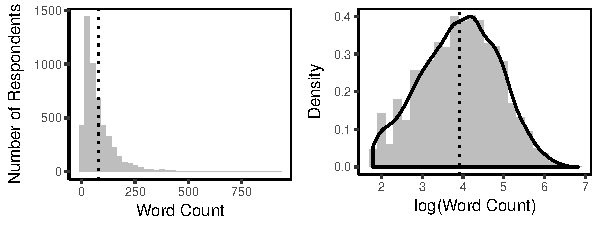
\includegraphics[width=\textwidth]{../calc/fig/app_wc.pdf}
\caption{Histograms displaying the distribution of individual response lengths in number of words for each respective item category. Dotted lines indicate the average response length.}\label{fig:appB2num}
\end{figure}

\begin{figure}[h]\centering
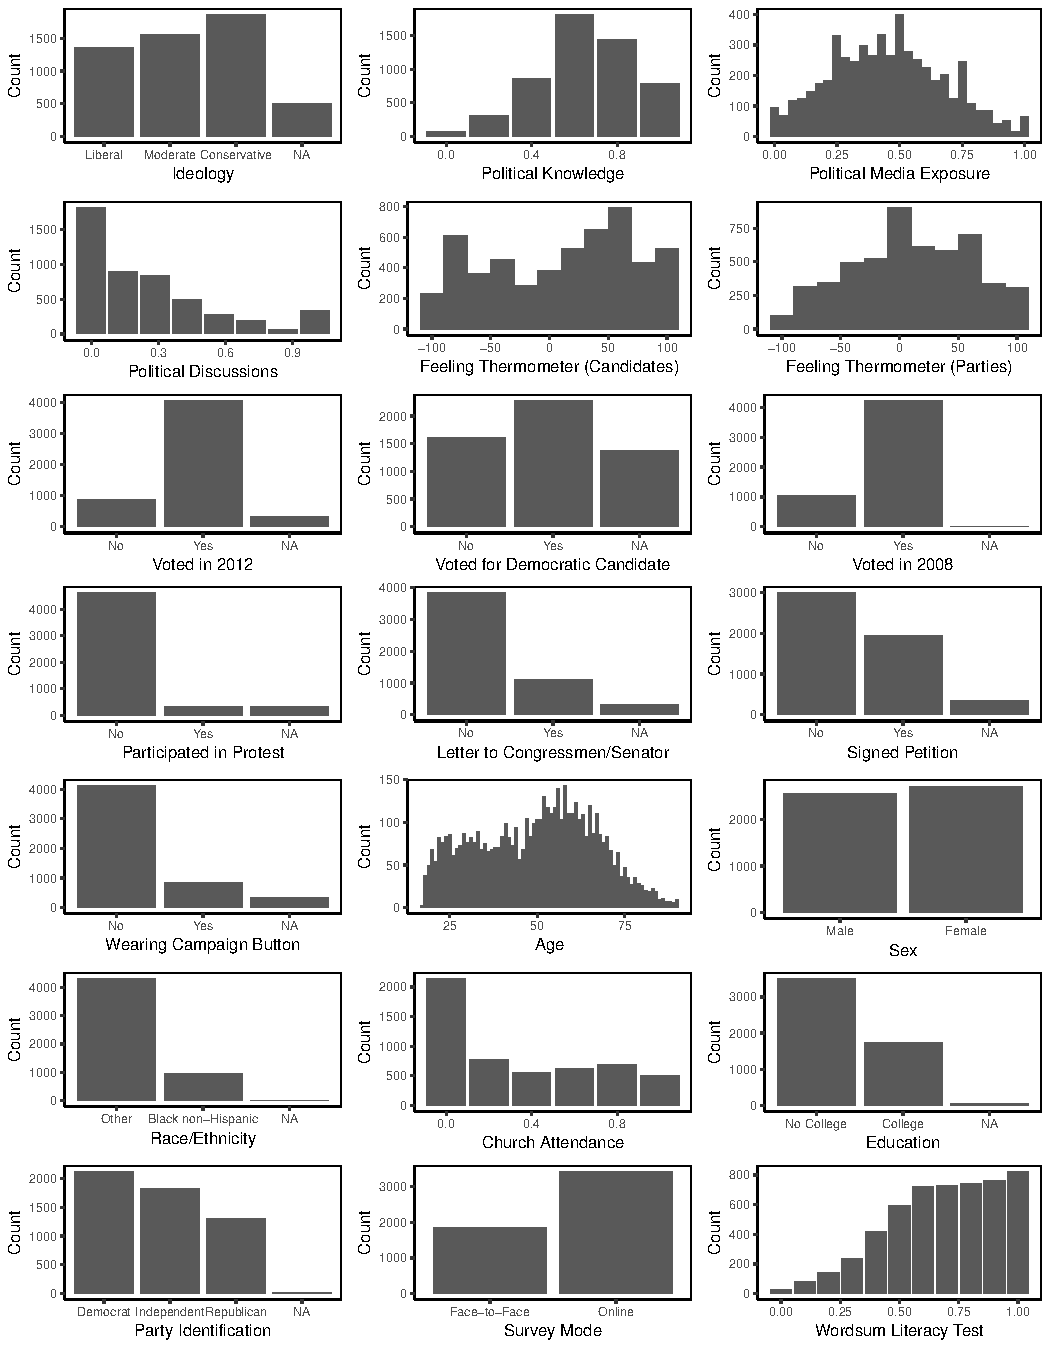
\includegraphics[width=\textwidth]{../calc/fig/app_desc.pdf}
\caption{Histograms for variables included in analyses.}\label{fig:app_desc}
\end{figure}

\begin{figure}[ht]\centering
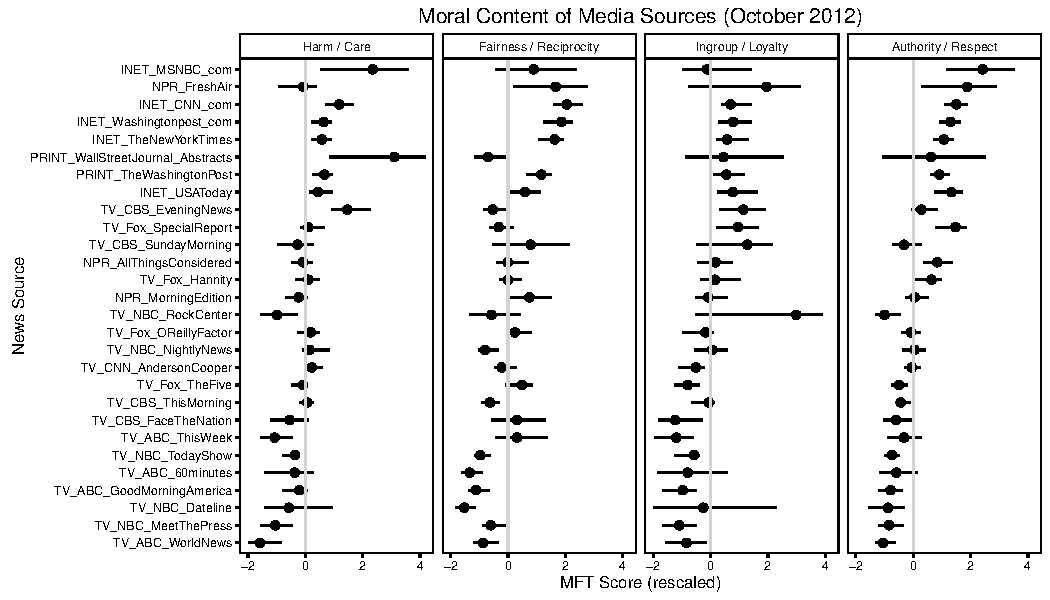
\includegraphics[width=\textwidth]{../calc/fig/media_desc.pdf}
\caption{MFT scores for media sources during 2012 U.S. Presidential campaign. Articles and scripts were selected if they mentioned either presidential candidate during the last month of the campaign (October). Contents were retrieved in full text from Lexis-Nexis (except for the Wall Street Journal, which only provided abstracts). Each media source was analyzed using the same procedure described for open-ended responses (weighted proportion of signal word occurrence for each foundation, c.f., equation~[\ref{eq:tfidf}]). Scores were median-centered and rescaled to unit variance. The figure also displays 95\% confidence intervals, which are based on parametric bootstraps of the document feature matrix of the entire corpus (500 iterations).}\label{fig:media_desc}
\end{figure}

\begin{figure}[h]\centering
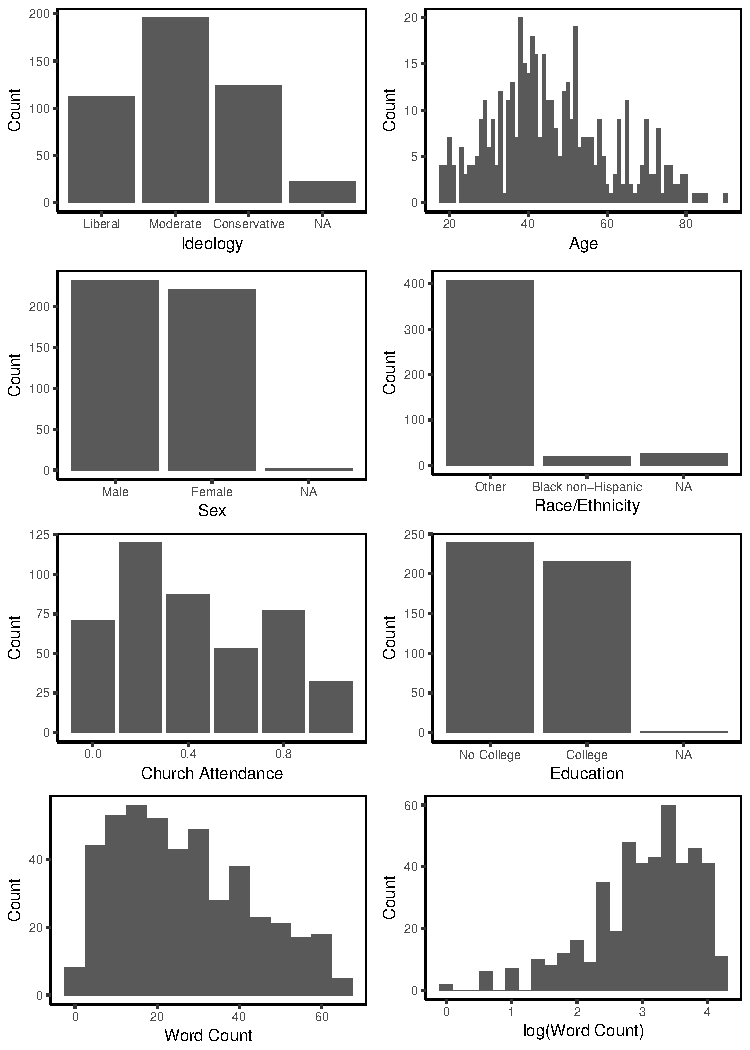
\includegraphics[width=.67\textwidth]{../calc/fig/app_lidesc.pdf}
\caption{Histograms for variables included in replication survey.}\label{fig:app_lidesc}
\end{figure}


\clearpage
\section{Additional Model Results and Robustness Checks}\label{app:robust}
\renewcommand\thefigure{\thesection.\arabic{figure}}
\renewcommand\thetable{\thesection.\arabic{table}}
\setcounter{figure}{0}
\setcounter{table}{0}


\begin{figure}[h]\centering
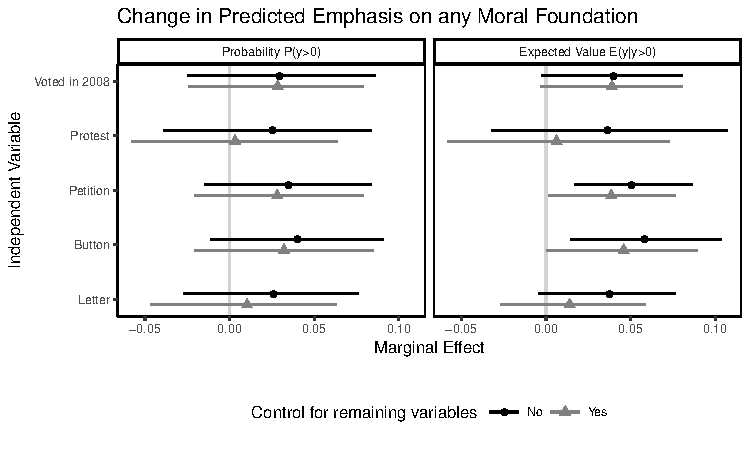
\includegraphics{../calc/fig/tobit_part.pdf}
\caption{Change in predicted overall reliance on moral foundations depending on previous turnout and non-conventional forms of participation (protest, petitions, campaign buttons, letter to congressmen/senator). The plot shows differences in predicted probabilities of mentioning any moral foundation (left panel) as well as in the summed MFT scores given that any foundation was mentioned (right panel), if a respondent engaged in the respective form of participation (vs. not) holding all other variables constant at their respective means (along with 95\% confidence intervals). Positive values indicate higher probability of mentioning, or stronger emphasis on moral foundations. Estimates are based on Tobit models and gray triangles indicate estimates while additionally controlling for the remaining variables presented in the figure. Full model results are displayed in the appendix, Table~\ref{tab:tobit_part}.
}\label{fig:tobit_part}
\end{figure}


\begin{figure}[ht]\centering
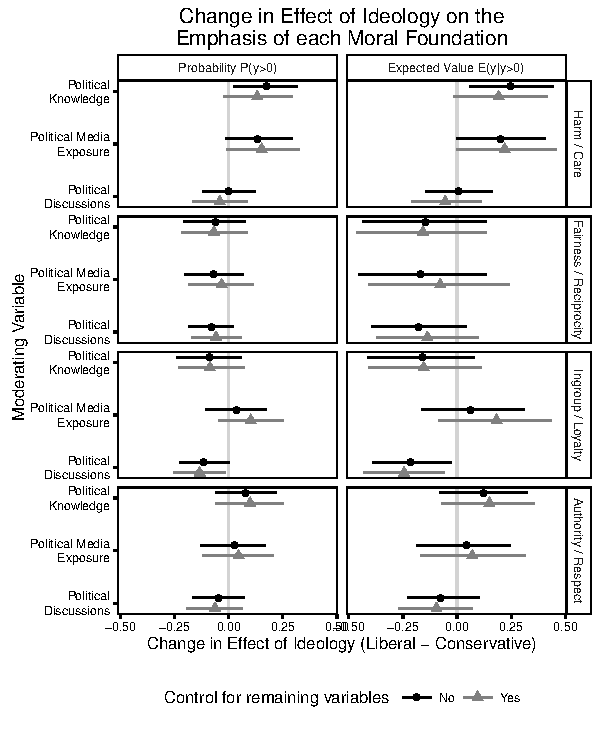
\includegraphics[scale=.8]{../calc/fig/tobit_ideol_difdif.pdf}
\caption{Change in effect of ideology on emphasis of each moral foundation moderated by political knowledge, media exposure, and frequency of political discussions (difference-in-difference). The plot shows how the difference between liberals and conservatives in predicted probabilities to mention each moral foundation, as well as the respective MFT scores, change if each of the independent variables is increased from its minimum to its maximum value holding control variables constant at their respective means (along with 95\% confidence intervals). Positive values indicate that liberals are more likely to mention a specific moral foundation if they score high on the moderating variable (knowledge, exposure, discussions, previous turnout, protest behavior), and vice versa. Estimates are based on individual Tobit models for each foundation and gray triangles indicate estimates while controlling for all remaining variables displayed in the figure. Full model results are displayed in Tables~\ref{tab:tobit_ideol_know}, \ref{tab:tobit_ideol_media}, \ref{tab:tobit_ideol_disc}, and \ref{tab:tobit_ideol_difdif}.
}\label{fig:tobit_ideol_difdif}
\end{figure}


\clearpage
\section{Tables of Model Estimates}\label{app:tables}
\renewcommand\thefigure{\thesection.\arabic{figure}}
\renewcommand\thetable{\thesection.\arabic{table}}
\setcounter{figure}{0}
\setcounter{table}{0}


\subsection*{Ideological Differences in Moral Reasoning}
% latex table generated in R 3.3.3 by xtable 1.8-2 package
% Tue Mar 14 22:58:48 2017
\begin{table}[ht]
\centering
\caption{Tobit models predicting MFT score for each foundation based 
           on ideology. Positive coefficients indicate stronger emphasis on the respective 
           foundation. Standard errors in parentheses. Estimates are used for Figure 
           \ref{fig:tobit_ideol} in the main text.} 
\label{tab:tobit_ideol}
\begingroup\footnotesize
\begin{tabular}{lcccc}
  \hline
Variable & Harm & Fairness & Ingroup & Authority \\ 
  \hline
Ideology (Conservative) & -0.307 & -0.697 &  0.366 & -0.132 \\ 
   & (0.08) & (0.143) & (0.115) & (0.091) \\ 
  Ideology (Moderate) & -0.135 & -0.513 &  0.099 & -0.060 \\ 
   & (0.081) & (0.146) & (0.121) & (0.093) \\ 
  Church Attendance & -0.063 &  0.110 &  0.247 & -0.123 \\ 
   & (0.092) & (0.167) & (0.132) & (0.105) \\ 
  Education (College Degree) & -0.093 &  0.237 &  0.308 &  0.106 \\ 
   & (0.07) & (0.125) & (0.099) & (0.079) \\ 
  Age &  0.002 &  0.001 & -0.007 &  0.003 \\ 
   & (0.002) & (0.004) & (0.003) & (0.002) \\ 
  Sex (Female) &  0.133 &  0.078 & -0.245 & -0.095 \\ 
   & (0.063) & (0.114) & (0.091) & (0.072) \\ 
  Race (African American) &  0.045 & -0.125 & -0.215 &  0.338 \\ 
   & (0.091) & (0.166) & (0.135) & (0.101) \\ 
  Word Count (log) &  0.364 &  0.527 &  0.773 &  0.584 \\ 
   & (0.033) & (0.061) & (0.051) & (0.039) \\ 
  Wordsum Score &  0.562 &  0.661 &  0.604 &  0.324 \\ 
   & (0.166) & (0.302) & (0.241) & (0.188) \\ 
  Survey Mode (Online) & -0.039 &  0.205 &  0.149 &  0.300 \\ 
   & (0.076) & (0.138) & (0.109) & (0.087) \\ 
  Intercept & -2.506 & -4.742 & -4.857 & -3.617 \\ 
   & (0.193) & (0.363) & (0.297) & (0.226) \\ 
  log(Sigma) &  0.553 &  1.025 &  0.868 &  0.684 \\ 
   & (0.021) & (0.027) & (0.023) & (0.02) \\ 
   \hline
N & 4684 & 4684 & 4684 & 4684 \\ 
  Log-Likelihood & -4924 & -3961 & -4567 & -5043 \\ 
   \hline
\end{tabular}
\endgroup
\end{table}


\clearpage
\subsection*{The Political Relevance of Moral Reasoning}
% latex table generated in R 3.3.3 by xtable 1.8-2 package
% Tue Mar 14 22:58:48 2017
\begin{table}[h]
\centering
\caption{OLS models predicting feeling thermometer differentials based on
           MFT score for each foundation. Positive coefficients indicate more favorable evaluation 
           of Democratic candidate/party than the Republican candidate/party, and vice versa. 
           Standard errors in parentheses. Estimates are used for Figure \ref{fig:ols_feel} 
           in the main text.} 
\label{tab:ols_feel}
\begingroup\footnotesize
\begin{tabular}{lcccc}
  \hline
Variable & Party (1) & Party (2) & Cand. (1) & Cand. (2) \\ 
  \hline
Harm &   2.558 &   0.781 &   2.798 &   0.907 \\ 
   & (0.714) & (0.5) & (0.855) & (0.642) \\ 
  Fairness &   1.833 &   0.692 &   3.095 &   1.793 \\ 
   & (0.623) & (0.435) & (0.748) & (0.56) \\ 
  Ingroup &  -2.919 &  -0.900 &  -4.009 &  -1.767 \\ 
   & (0.647) & (0.452) & (0.777) & (0.583) \\ 
  Authority &   2.214 &   0.503 &   2.209 &   0.338 \\ 
   & (0.669) & (0.468) & (0.796) & (0.597) \\ 
  PID (Democrat) &  &  44.602 &  &  47.207 \\ 
   &  & (1.074) &  & (1.375) \\ 
  PID (Republican) &  & -44.706 &  & -52.275 \\ 
   &  & (1.189) &  & (1.527) \\ 
  Church Attendance & -27.658 & -11.449 & -35.883 & -17.639 \\ 
   & (1.82) & (1.296) & (2.18) & (1.666) \\ 
  Education (College Degree) &   0.310 &   1.311 &   1.361 &   2.525 \\ 
   & (1.464) & (1.023) & (1.756) & (1.317) \\ 
  Age &  -0.109 &  -0.119 &  -0.307 &  -0.316 \\ 
   & (0.039) & (0.028) & (0.047) & (0.035) \\ 
  Sex (Female) &   7.475 &   2.939 &   9.280 &   4.383 \\ 
   & (1.279) & (0.897) & (1.532) & (1.152) \\ 
  Race (African American) &  52.935 &  20.983 &  63.106 &  28.211 \\ 
   & (1.739) & (1.294) & (2.08) & (1.659) \\ 
  Word Count (log) &   2.308 &   1.089 &   1.758 &   0.335 \\ 
   & (0.636) & (0.445) & (0.762) & (0.571) \\ 
  Wordsum Score &  -0.862 &   2.579 &   0.553 &   4.125 \\ 
   & (3.297) & (2.309) & (3.955) & (2.971) \\ 
  Survey Mode (Online) &  -5.829 &  -1.986 &  -8.684 &  -4.467 \\ 
   & (1.511) & (1.06) & (1.808) & (1.362) \\ 
  Intercept &   8.242 &   4.708 &  21.501 &  19.260 \\ 
   & (3.346) & (2.385) & (4.002) & (3.056) \\ 
   \hline
N & 5135 & 5123 & 5151 & 5140 \\ 
  R-squared (adj.) & 0.211 & 0.616 & 0.224 & 0.565 \\ 
   \hline
\end{tabular}
\endgroup
\end{table}

% latex table generated in R 3.4.2 by xtable 1.8-2 package
% Sat Nov 25 14:03:51 2017
\begin{table}[ht]
\centering
\caption{Logit models predicting democratic vote choice based on
           MFT score for each foundation. Positive coefficients indicate higher likelihood
           to vote for the Democratic candidate than the Republican candidate. Standard errors 
           in parentheses. Estimates are used for Figure 2 in the main text.} 
\label{tab:logit_vote}
\begingroup\footnotesize
\begin{tabular}{lcc}
  \hline
Variable & (1) & (2) \\ 
  \hline
Harm &  0.192 &  0.171 \\ 
   & (0.043) & (0.061) \\ 
  Fairness &  0.170 &  0.129 \\ 
   & (0.041) & (0.053) \\ 
  Ingroup & -0.190 & -0.068 \\ 
   & (0.041) & (0.054) \\ 
  Authority &  0.076 &  0.025 \\ 
   & (0.041) & (0.056) \\ 
  PID (Democrat) &  &  2.618 \\ 
   &  & (0.136) \\ 
  PID (Republican) &  & -2.676 \\ 
   &  & (0.156) \\ 
  Church Attendance & -1.614 & -1.352 \\ 
   & (0.113) & (0.158) \\ 
  Education (College Degree) &  0.155 &  0.370 \\ 
   & (0.085) & (0.119) \\ 
  Age & -0.009 & -0.017 \\ 
   & (0.002) & (0.003) \\ 
  Sex (Female) &  0.275 &  0.160 \\ 
   & (0.078) & (0.108) \\ 
  Race (African American) &  4.229 &  3.234 \\ 
   & (0.263) & (0.288) \\ 
  Word Count (log) &  0.145 &  0.116 \\ 
   & (0.044) & (0.061) \\ 
  Wordsum Score &  0.048 &  0.174 \\ 
   & (0.21) & (0.29) \\ 
  Survey Mode (Online) & -0.366 & -0.388 \\ 
   & (0.095) & (0.131) \\ 
  Intercept &  0.313 &  0.509 \\ 
   & (0.238) & (0.328) \\ 
   \hline
N & 3706 & 3698 \\ 
  Log-Likelihood & -1955 & -1138 \\ 
   \hline
\end{tabular}
\endgroup
\end{table}


\clearpage
\subsection*{The Conditionality of Moral Reasoning}
% latex table generated in R 3.3.0 by xtable 1.8-2 package
% Thu Nov 10 12:04:38 2016
\begin{table}[ht]
\centering
\caption{Tobit models predicting overall reliance on moral foundations
           (sum of MFT scores) based on political knowledge, media exposure, and frequency of 
           political discussions. Positive coefficients indicate stronger emphasis on any foundation.
           Standard errors in parentheses. Estimates are used for Figure \ref{fig:tobit_learn} in 
           the main text.} 
\label{tab:tobit_learn}
\begingroup\footnotesize
\begin{tabular}{lcccc}
  \hline
Variable & (1) & (2) & (3) & (4) \\ 
  \hline
Political Knowledge &  0.260 &  &  &  0.236 \\ 
   & (0.098) &  &  & (0.103) \\ 
  Political Media Exposure &  &  0.369 &  &  0.272 \\ 
   &  & (0.088) &  & (0.095) \\ 
  Political
Discussions &  &  &  0.263 &  0.202 \\ 
   &  &  & (0.068) & (0.07) \\ 
  Church Attendance & -0.020 & -0.022 & -0.006 & -0.010 \\ 
   & (0.052) & (0.053) & (0.055) & (0.055) \\ 
  Education (College Degree) &  0.079 &  0.079 &  0.097 &  0.070 \\ 
   & (0.043) & (0.042) & (0.044) & (0.044) \\ 
  Age & -0.001 & -0.002 &  0.000 & -0.002 \\ 
   & (0.001) & (0.001) & (0.001) & (0.001) \\ 
  Sex (Female) &  0.018 &  0.016 &  0.017 &  0.041 \\ 
   & (0.037) & (0.037) & (0.038) & (0.039) \\ 
  Race (African American) &  0.109 &  0.088 &  0.082 &  0.091 \\ 
   & (0.05) & (0.05) & (0.052) & (0.052) \\ 
  Word Count (log) &  0.099 &  0.097 &  0.090 &  0.080 \\ 
   & (0.019) & (0.018) & (0.019) & (0.02) \\ 
  Wordsum Score &  0.281 &  0.353 &  0.323 &  0.257 \\ 
   & (0.1) & (0.096) & (0.1) & (0.104) \\ 
  Survey Mode (Online) &  0.042 &  0.043 &  0.099 &  0.061 \\ 
   & (0.044) & (0.044) & (0.046) & (0.047) \\ 
  Intercept & -0.401 & -0.380 & -0.356 & -0.446 \\ 
   & (0.1) & (0.097) & (0.101) & (0.105) \\ 
  log(Sigma) &  0.209 &  0.209 &  0.213 &  0.212 \\ 
   & (0.014) & (0.014) & (0.014) & (0.014) \\ 
   \hline
N & 5173 & 5164 & 4834 & 4827 \\ 
  Log-Likelihood & -7132 & -7117 & -6687 & -6672 \\ 
   \hline
\end{tabular}
\endgroup
\end{table}

% latex table generated in R 3.3.3 by xtable 1.8-2 package
% Sun Mar 19 13:46:11 2017
\begin{table}[ht]
\centering
\caption{Tobit models predicting MFT score for each foundation based 
           on political knowledge (mean-centered) and ideology. Positive coefficients indicate stronger 
           emphasis on the respective foundation. Standard errors in parentheses. Estimates are used 
           for Figure \ref{fig:tobit_ideol_know} in the main text.} 
\label{tab:tobit_ideol_know}
\begingroup\footnotesize
\begin{tabular}{lcccc}
  \hline
Variable & Harm & Fairness & Ingroup & Authority \\ 
  \hline
Political Knowledge &  0.795 & -0.236 & -0.037 &  0.882 \\ 
   & (0.299) & (0.472) & (0.406) & (0.312) \\ 
  Ideology (Conservative) & -0.325 & -0.866 &  0.340 & -0.092 \\ 
   & (0.092) & (0.152) & (0.123) & (0.096) \\ 
  Knowledge * Conservative & -0.984 &  0.780 &  0.551 & -0.596 \\ 
   & (0.388) & (0.632) & (0.511) & (0.4) \\ 
  Ideology (Moderate) & -0.190 & -0.730 &  0.044 & -0.003 \\ 
   & (0.091) & (0.15) & (0.125) & (0.095) \\ 
  Knowledge * Moderate & -0.503 &  0.653 &  0.136 & -1.077 \\ 
   & (0.405) & (0.667) & (0.552) & (0.417) \\ 
  Church Attendance &  0.014 &  0.066 &  0.255 & -0.105 \\ 
   & (0.103) & (0.169) & (0.134) & (0.105) \\ 
  Education (College Degree) & -0.129 &  0.280 &  0.328 &  0.078 \\ 
   & (0.079) & (0.128) & (0.102) & (0.08) \\ 
  Age &  0.000 &  0.001 & -0.008 &  0.002 \\ 
   & (0.002) & (0.004) & (0.003) & (0.002) \\ 
  Sex (Female) &  0.107 &  0.139 & -0.204 & -0.088 \\ 
   & (0.071) & (0.118) & (0.094) & (0.073) \\ 
  Race (African American) &  0.123 & -0.033 & -0.236 &  0.353 \\ 
   & (0.101) & (0.169) & (0.139) & (0.102) \\ 
  Word Count (log) &  0.410 &  0.601 &  0.751 &  0.492 \\ 
   & (0.041) & (0.068) & (0.055) & (0.042) \\ 
  Wordsum Score &  0.659 &  0.721 &  0.547 &  0.221 \\ 
   & (0.193) & (0.321) & (0.256) & (0.197) \\ 
  Survey Mode (Online) & -0.054 &  0.294 &  0.130 &  0.266 \\ 
   & (0.085) & (0.141) & (0.112) & (0.088) \\ 
  Intercept & -2.575 & -4.962 & -4.664 & -3.133 \\ 
   & (0.236) & (0.403) & (0.325) & (0.246) \\ 
  log(Sigma) &  0.669 &  1.045 &  0.884 &  0.683 \\ 
   & (0.02) & (0.026) & (0.022) & (0.02) \\ 
   \hline
N & 4489 & 4489 & 4489 & 4489 \\ 
  Log-Likelihood & -5144 & -3983 & -4579 & -5025 \\ 
   \hline
\end{tabular}
\endgroup
\end{table}

% latex table generated in R 3.3.2 by xtable 1.8-2 package
% Mon Feb 27 15:07:15 2017
\begin{table}[ht]
\centering
\caption{Tobit models predicting MFT score for each foundation based 
           on political media exposure (mean-centered) and ideology. Positive coefficients indicate 
           stronger emphasis on the respective foundation. Standard errors in parentheses. Estimates 
           are used for Figure \ref{fig:tobit_ideol_media} in the main text.} 
\label{tab:tobit_ideol_media}
\begingroup\footnotesize
\begin{tabular}{lcccc}
  \hline
Variable & Harm & Fairness & Ingroup & Authority \\ 
  \hline
Political Media Exposure &  0.557 &  0.113 &  0.678 &  0.773 \\ 
   & (0.262) & (0.46) & (0.394) & (0.302) \\ 
  Ideology (Conservative) & -0.281 & -0.731 &  0.379 & -0.123 \\ 
   & (0.081) & (0.146) & (0.117) & (0.093) \\ 
  Media * Conservative & -0.651 &  0.811 & -0.385 & -0.177 \\ 
   & (0.341) & (0.606) & (0.491) & (0.388) \\ 
  Ideology (Moderate) & -0.122 & -0.508 &  0.121 & -0.034 \\ 
   & (0.081) & (0.146) & (0.122) & (0.093) \\ 
  Media * Moderate & -0.383 &  0.041 & -0.507 & -0.691 \\ 
   & (0.35) & (0.629) & (0.525) & (0.402) \\ 
  Church Attendance & -0.066 &  0.113 &  0.249 & -0.124 \\ 
   & (0.092) & (0.167) & (0.132) & (0.105) \\ 
  Education (College Degree) & -0.108 &  0.226 &  0.293 &  0.079 \\ 
   & (0.07) & (0.126) & (0.1) & (0.079) \\ 
  Age &  0.001 & -0.001 & -0.009 &  0.000 \\ 
   & (0.002) & (0.004) & (0.003) & (0.002) \\ 
  Sex (Female) &  0.139 &  0.102 & -0.231 & -0.069 \\ 
   & (0.063) & (0.115) & (0.092) & (0.072) \\ 
  Race (African American) &  0.032 & -0.122 & -0.217 &  0.322 \\ 
   & (0.091) & (0.167) & (0.135) & (0.102) \\ 
  Word Count (log) &  0.359 &  0.520 &  0.765 &  0.576 \\ 
   & (0.033) & (0.061) & (0.051) & (0.039) \\ 
  Wordsum Score &  0.563 &  0.650 &  0.623 &  0.322 \\ 
   & (0.166) & (0.302) & (0.242) & (0.188) \\ 
  Survey Mode (Online) & -0.049 &  0.189 &  0.132 &  0.284 \\ 
   & (0.076) & (0.139) & (0.11) & (0.088) \\ 
  Intercept & -2.445 & -4.616 & -4.762 & -3.480 \\ 
   & (0.199) & (0.371) & (0.305) & (0.232) \\ 
  log(Sigma) &  0.553 &  1.025 &  0.868 &  0.684 \\ 
   & (0.021) & (0.027) & (0.023) & (0.02) \\ 
   \hline
N & 4678 & 4678 & 4678 & 4678 \\ 
  Log-Likelihood & -4916 & -3955 & -4561 & -5034 \\ 
   \hline
\end{tabular}
\endgroup
\end{table}

% latex table generated in R 3.3.0 by xtable 1.8-2 package
% Thu Nov 10 12:04:39 2016
\begin{table}[ht]
\centering
\caption{Tobit models predicting MFT score for each foundation based 
           on political discussion frequency (mean-centered) and ideology. Positive coefficients 
           indicate stronger emphasis on the respective foundation. Standard errors in parentheses. 
           Estimates are used for Figure \ref{fig:tobit_ideol_disc} in the main text.} 
\label{tab:tobit_ideol_disc}
\begingroup\footnotesize
\begin{tabular}{lcccc}
  \hline
Variable & Harm & Fairness & Ingroup & Authority \\ 
  \hline
Political Discussion &  0.149 &  0.182 &  0.178 &  0.222 \\ 
   & (0.182) & (0.341) & (0.282) & (0.216) \\ 
  Ideology (Conservative) & -0.283 & -0.727 &  0.276 & -0.122 \\ 
   & (0.079) & (0.153) & (0.12) & (0.094) \\ 
  Discussion * Conservative &  0.132 &  0.683 &  0.717 &  0.242 \\ 
   & (0.238) & (0.45) & (0.356) & (0.28) \\ 
  Ideology (Moderate) & -0.157 & -0.497 &  0.090 & -0.090 \\ 
   & (0.079) & (0.153) & (0.124) & (0.094) \\ 
  Discussion * Moderate & -0.356 &  0.729 &  0.576 & -0.547 \\ 
   & (0.27) & (0.507) & (0.41) & (0.322) \\ 
  Church Attendance &  0.001 &  0.126 &  0.265 & -0.149 \\ 
   & (0.09) & (0.174) & (0.135) & (0.106) \\ 
  Education (College Degree) & -0.074 &  0.222 &  0.308 &  0.119 \\ 
   & (0.068) & (0.13) & (0.101) & (0.08) \\ 
  Age & -0.002 &  0.000 & -0.007 &  0.003 \\ 
   & (0.002) & (0.004) & (0.003) & (0.002) \\ 
  Sex (Female) &  0.158 &  0.124 & -0.240 & -0.070 \\ 
   & (0.061) & (0.119) & (0.093) & (0.073) \\ 
  Race (African American) &  0.003 & -0.135 & -0.228 &  0.338 \\ 
   & (0.088) & (0.173) & (0.138) & (0.103) \\ 
  Word Count (log) &  0.311 &  0.474 &  0.730 &  0.557 \\ 
   & (0.033) & (0.064) & (0.053) & (0.04) \\ 
  Wordsum Score &  0.530 &  0.698 &  0.550 &  0.342 \\ 
   & (0.162) & (0.317) & (0.249) & (0.192) \\ 
  Survey Mode (Online) & -0.079 &  0.251 &  0.219 &  0.283 \\ 
   & (0.074) & (0.145) & (0.113) & (0.089) \\ 
  Intercept & -1.972 & -4.605 & -4.670 & -3.526 \\ 
   & (0.188) & (0.383) & (0.308) & (0.234) \\ 
  log(Sigma) &  0.509 &  1.033 &  0.856 &  0.665 \\ 
   & (0.021) & (0.028) & (0.023) & (0.021) \\ 
   \hline
N & 4377 & 4377 & 4377 & 4377 \\ 
  Log-Likelihood & -4812 & -3727 & -4271 & -4726 \\ 
   \hline
\end{tabular}
\endgroup
\end{table}

% latex table generated in R 3.3.0 by xtable 1.8-2 package
% Thu Nov 10 12:04:39 2016
\begin{table}[ht]
\centering
\caption{Tobit models predicting MFT score for each foundation based 
           on moral content of individual media environments. Positive coefficients 
           indicate stronger emphasis on the respective foundation. Standard errors in parentheses. 
           Estimates are used for Figure \ref{fig:tobit_cont} in the main text.} 
\label{tab:tobit_cont}
\begingroup\footnotesize
\begin{tabular}{lcccc}
  \hline
Variable & Harm & Fairness & Ingroup & Authority \\ 
  \hline
Media MFT score (harm) &  0.030 &  &  &  \\ 
   & (0.016) &  &  &  \\ 
  Media MFT score (fairness) &  &  0.051 &  &  \\ 
   &  & (0.024) &  &  \\ 
  Media MFT score (ingroup) &  &  &  0.001 &  \\ 
   &  &  & (0.029) &  \\ 
  Media MFT score (authority) &  &  &  &  0.001 \\ 
   &  &  &  & (0.017) \\ 
  Church Attendance & -0.128 & -0.029 &  0.357 & -0.115 \\ 
   & (0.078) & (0.152) & (0.124) & (0.097) \\ 
  Education (College Degree) & -0.063 &  0.239 &  0.345 &  0.110 \\ 
   & (0.063) & (0.122) & (0.099) & (0.079) \\ 
  Age & -0.002 &  0.002 & -0.004 &  0.001 \\ 
   & (0.002) & (0.003) & (0.003) & (0.002) \\ 
  Sex (Female) &  0.196 &  0.153 & -0.308 & -0.092 \\ 
   & (0.055) & (0.109) & (0.088) & (0.069) \\ 
  Race (African American) &  0.161 & -0.020 & -0.272 &  0.383 \\ 
   & (0.073) & (0.15) & (0.123) & (0.092) \\ 
  Word Count (log) &  0.304 &  0.560 &  0.798 &  0.588 \\ 
   & (0.028) & (0.058) & (0.049) & (0.037) \\ 
  Wordsum Score &  0.519 &  0.679 &  0.452 &  0.255 \\ 
   & (0.143) & (0.288) & (0.233) & (0.181) \\ 
  Survey Mode (Online) & -0.117 &  0.322 &  0.248 &  0.268 \\ 
   & (0.064) & (0.128) & (0.104) & (0.081) \\ 
  Intercept & -2.025 & -5.414 & -4.945 & -3.535 \\ 
   & (0.152) & (0.331) & (0.269) & (0.201) \\ 
  log(Sigma) &  0.481 &  1.011 &  0.879 &  0.691 \\ 
   & (0.019) & (0.026) & (0.022) & (0.019) \\ 
   \hline
N & 5173 & 5173 & 5173 & 5173 \\ 
  Log-Likelihood & -5650 & -4222 & -4936 & -5581 \\ 
   \hline
\end{tabular}
\endgroup
\end{table}


\clearpage
\subsection*{Examining Alternative Explanations}
% latex table generated in R 3.3.0 by xtable 1.8-2 package
% Thu Nov  3 19:42:25 2016
\begin{table}[ht]
\centering
\caption{Tobit models predicting MFT score for each foundation based 
           on ideology (telephone survey replication). Positive coefficients indicate stronger emphasis on the respective 
           foundation. Standard errors in parentheses. Estimates are used for Figure 
           \ref{fig:tobit_ideol_lisurvey} in the main text.} 
\label{tab:tobit_ideol_lisurvey}
\begingroup\footnotesize
\begin{tabular}{lcccc}
  \hline
Variable & Harm & Fairness & Ingroup & Authority \\ 
  \hline
Ideology (Conservative) &  -2.451 & -3.497 &   1.786 & -0.993 \\ 
   & (1.102) & (1.196) & (1.123) & (0.808) \\ 
  Ideology (Moderate) &  -1.374 & -1.917 &  -1.394 & -1.030 \\ 
   & (0.876) & (0.859) & (1.096) & (0.687) \\ 
  Church Attendance &  -0.918 &  1.363 &   1.015 &  1.455 \\ 
   & (1.282) & (1.25) & (1.375) & (0.977) \\ 
  Education (College Degree) &   0.810 &  0.482 &   1.197 &  1.100 \\ 
   & (0.787) & (0.762) & (0.885) & (0.606) \\ 
  Age &  -0.002 &  0.044 &  -0.031 & -0.058 \\ 
   & (0.026) & (0.025) & (0.029) & (0.022) \\ 
  Sex (Female) &  -0.777 & -0.097 &  -0.706 & -0.400 \\ 
   & (0.774) & (0.753) & (0.853) & (0.587) \\ 
  Race (African American) &   0.591 &  1.563 &  -0.038 &  0.385 \\ 
   & (1.731) & (1.598) & (2.107) & (1.305) \\ 
  Word Count (log) &   2.517 &  0.269 &   1.562 &  0.728 \\ 
   & (0.671) & (0.481) & (0.645) & (0.399) \\ 
  Intercept & -11.759 & -7.623 & -10.262 & -3.802 \\ 
   & (2.794) & (2.249) & (2.803) & (1.652) \\ 
  log(Sigma) &   1.507 &  1.433 &   1.595 &  1.325 \\ 
   & (0.121) & (0.139) & (0.127) & (0.108) \\ 
   \hline
N & 395 & 395 & 395 & 395 \\ 
  Log-Likelihood & -224 & -192 & -219 & -266 \\ 
   \hline
\end{tabular}
\endgroup
\end{table}


\clearpage
\subsection*{Additional Models and Robustness Checks in Appendix}
% latex table generated in R 3.3.0 by xtable 1.8-2 package
% Thu Nov  3 16:40:24 2016
\begin{table}[ht]
\centering
\caption{Tobit models predicting overall reliance on moral foundations
           (sum of MFT scores) based on political participation. Positive coefficients indicate 
           stronger emphasis on any foundation. Standard errors in parentheses. Estimates are 
           used for Figure \ref{fig:tobit_part} in the appendix.} 
\label{tab:tobit_part}
\begingroup\footnotesize
\begin{tabular}{lcccccc}
  \hline
Variable & (1) & (2) & (3) & (4) & (5) & (6) \\ 
  \hline
Voted in 2008 &  0.096 &  &  &  &  &  0.091 \\ 
   & (0.052) &  &  &  &  & (0.054) \\ 
  Protest &  &  0.076 &  &  &  & -0.002 \\ 
   &  & (0.076) &  &  &  & (0.08) \\ 
  Petition &  &  &  0.122 &  &  &  0.091 \\ 
   &  &  & (0.041) &  &  & (0.044) \\ 
  Button &  &  &  &  0.135 &  &  0.106 \\ 
   &  &  &  & (0.051) &  & (0.052) \\ 
  Letter &  &  &  &  &  0.090 &  0.040 \\ 
   &  &  &  &  & (0.048) & (0.051) \\ 
  Church Attendance & -0.032 &  0.001 &  0.001 & -0.007 & -0.004 & -0.023 \\ 
   & (0.053) & (0.055) & (0.055) & (0.055) & (0.055) & (0.055) \\ 
  Education (College Degree) &  0.085 &  0.103 &  0.095 &  0.108 &  0.095 &  0.086 \\ 
   & (0.043) & (0.044) & (0.044) & (0.044) & (0.044) & (0.045) \\ 
  Age & -0.001 &  0.000 &  0.000 &  0.000 &  0.000 & -0.001 \\ 
   & (0.001) & (0.001) & (0.001) & (0.001) & (0.001) & (0.001) \\ 
  Sex (Female) &  0.002 &  0.011 &  0.010 &  0.010 &  0.015 &  0.014 \\ 
   & (0.037) & (0.038) & (0.038) & (0.038) & (0.038) & (0.039) \\ 
  Race (African American) &  0.089 &  0.088 &  0.090 &  0.069 &  0.092 &  0.071 \\ 
   & (0.05) & (0.052) & (0.052) & (0.052) & (0.052) & (0.053) \\ 
  Word Count (log) &  0.103 &  0.105 &  0.097 &  0.103 &  0.101 &  0.091 \\ 
   & (0.018) & (0.019) & (0.019) & (0.019) & (0.019) & (0.02) \\ 
  Wordsum Score &  0.339 &  0.349 &  0.312 &  0.350 &  0.338 &  0.299 \\ 
   & (0.096) & (0.1) & (0.101) & (0.1) & (0.1) & (0.101) \\ 
  Survey Mode (Online) &  0.053 &  0.080 &  0.070 &  0.073 &  0.069 &  0.056 \\ 
   & (0.044) & (0.045) & (0.046) & (0.045) & (0.046) & (0.046) \\ 
  Intercept & -0.353 & -0.385 & -0.362 & -0.376 & -0.358 & -0.364 \\ 
   & (0.097) & (0.101) & (0.102) & (0.101) & (0.102) & (0.103) \\ 
  log(Sigma) &  0.209 &  0.215 &  0.215 &  0.214 &  0.214 &  0.213 \\ 
   & (0.014) & (0.014) & (0.014) & (0.014) & (0.014) & (0.014) \\ 
   \hline
N & 5157 & 4846 & 4833 & 4849 & 4847 & 4816 \\ 
  Log-Likelihood & -7108 & -6709 & -6688 & -6709 & -6709 & -6657 \\ 
   \hline
\end{tabular}
\endgroup
\end{table}

% latex table generated in R 3.3.3 by xtable 1.8-2 package
% Tue Mar 14 22:58:50 2017
\begin{table}[ht]
\centering
\caption{Tobit models predicting MFT score for each foundation based 
           on political knowledge, media exposure, and discussion frequency (all mean-centered)
           as well as ideology. Positive coefficients indicate stronger emphasis on the respective
           foundation. Standard errors in parentheses. Estimates are used for Figure
           \ref{fig:tobit_ideol_difdif} in the appendix.} 
\label{tab:tobit_ideol_difdif}
\begingroup\footnotesize
\begin{tabular}{lcccc}
  \hline
Variable & Harm & Fairness & Ingroup & Authority \\ 
  \hline
Political Knowledge &  0.671 & -0.188 & -0.093 &  0.789 \\ 
   & (0.28) & (0.492) & (0.407) & (0.315) \\ 
  Political Media Exposure &  0.465 & -0.034 &  0.602 &  0.588 \\ 
   & (0.284) & (0.502) & (0.417) & (0.319) \\ 
  Political Discussion &  0.049 &  0.200 &  0.057 &  0.081 \\ 
   & (0.202) & (0.356) & (0.295) & (0.226) \\ 
  Ideology (Conservative) & -0.291 & -0.774 &  0.259 & -0.066 \\ 
   & (0.088) & (0.16) & (0.125) & (0.098) \\ 
  Knowledge * Conservative & -0.661 &  0.524 &  0.516 & -0.687 \\ 
   & (0.373) & (0.671) & (0.524) & (0.413) \\ 
  Media * Conservative & -0.720 &  0.429 & -0.777 & -0.174 \\ 
   & (0.378) & (0.675) & (0.533) & (0.418) \\ 
  Discussion * Conservative &  0.204 &  0.540 &  0.855 &  0.300 \\ 
   & (0.267) & (0.474) & (0.375) & (0.294) \\ 
  Ideology (Moderate) & -0.129 & -0.496 &  0.075 & -0.038 \\ 
   & (0.086) & (0.154) & (0.126) & (0.096) \\ 
  Knowledge * Moderate & -0.372 & -0.366 &  0.779 & -0.945 \\ 
   & (0.38) & (0.685) & (0.561) & (0.425) \\ 
  Media * Moderate & -0.183 &  0.017 & -0.592 & -0.350 \\ 
   & (0.38) & (0.69) & (0.562) & (0.427) \\ 
  Discussion * Moderate & -0.298 &  0.736 &  0.661 & -0.418 \\ 
   & (0.298) & (0.526) & (0.425) & (0.334) \\ 
  Church Attendance & -0.009 &  0.123 &  0.255 & -0.146 \\ 
   & (0.096) & (0.174) & (0.135) & (0.106) \\ 
  Education (College Degree) & -0.151 &  0.228 &  0.287 &  0.076 \\ 
   & (0.074) & (0.132) & (0.103) & (0.081) \\ 
  Age &  0.000 & -0.001 & -0.008 &  0.001 \\ 
   & (0.002) & (0.004) & (0.003) & (0.002) \\ 
  Sex (Female) &  0.141 &  0.128 & -0.211 & -0.039 \\ 
   & (0.067) & (0.121) & (0.095) & (0.074) \\ 
  Race (African American) &  0.024 & -0.137 & -0.211 &  0.346 \\ 
   & (0.095) & (0.175) & (0.139) & (0.103) \\ 
  Word Count (log) &  0.350 &  0.478 &  0.718 &  0.546 \\ 
   & (0.035) & (0.065) & (0.053) & (0.04) \\ 
  Wordsum Score &  0.466 &  0.738 &  0.479 &  0.285 \\ 
   & (0.18) & (0.33) & (0.258) & (0.199) \\ 
  Survey Mode (Online) & -0.066 &  0.247 &  0.183 &  0.243 \\ 
   & (0.081) & (0.148) & (0.115) & (0.09) \\ 
  Intercept & -2.314 & -4.623 & -4.496 & -3.358 \\ 
   & (0.216) & (0.406) & (0.323) & (0.246) \\ 
  log(Sigma) &  0.556 &  1.033 &  0.855 &  0.663 \\ 
   & (0.021) & (0.028) & (0.023) & (0.021) \\ 
   \hline
N & 4372 & 4372 & 4372 & 4372 \\ 
  Log-Likelihood & -4624 & -3722 & -4266 & -4712 \\ 
   \hline
\end{tabular}
\endgroup
\end{table}




\end{document}